%----------------------------------------------------------------------------------------
%	PACKAGES AND THEMES
%----------------------------------------------------------------------------------------
\PassOptionsToPackage{table}{xcolor}
\documentclass[aspectratio=169,xcolor=dvipsnames,11pt]{beamer}
\usetheme{SimplePlusAIC}
\usepackage{amsmath}

\usepackage{hyperref}
\usepackage{cleveref}
\usepackage{caption}
\usepackage{graphicx} % Allows including images
\usepackage{subfig}
\usepackage{booktabs} % Allows the use of \toprule, \midrule and  \bottomrule in tables
\usepackage{svg} %allows using svg figures
\usepackage{tikz}
\usepackage{makecell}
\usepackage{multirow}
\usepackage{wrapfig}
%\usepackage[dvipsnames]{xcolor}

\usepackage{hhline}
\usepackage{relsize}
\usepackage{bm}
%Select the Epilogue font (requires luaLatex or XeLaTex compilers)
%\setsansfont{Epilogue}[
  %  Path=./epilogueFont/,
  %  Scale=0.9,
  %  Extension = .ttf,
   % UprightFont=*-Regular,
   % BoldFont=*-Bold,
   % ItalicFont=*-Italic,
    %BoldItalicFont=*-BoldItalic
    %]
    \usefonttheme[onlymath]{serif}
% \usepackage{ eulervm } % Euler VM as math serif font

\newcommand*{\defeq}{\stackrel{\text{def}}{=}}
\newcommand{\grad}{\nabla}
\newcommand{\lap}{\Delta}
\newcommand{\weaklyto}{\rightharpoonup}
\newcommand{\weakstar}{\stackrel{*}\rightharpoonup}
\newcommand{\cts}{\hookrightarrow}
\newcommand{\ctsDense}{\xhookrightarrow{d}}
\newcommand{\ctsCompact}{\xhookrightarrow{c}}
\newcommand{\E}{\mathbb{E}}
\newcommand{\pP}{\mathbb{P}}
\newcommand{\R}{\mathbb{R}}
\newcommand{\ER}{\overline{\mathbb{R}}}
\newcommand{\cR}{\mathcal{R}}
\newcommand{\cJ}{\mathcal{J}}
\newcommand{\cG}{\mathcal{G}}
\newcommand{\CVaR}{\textup{CVaR}}
\newcommand{\D}{\textup{ d}}
\newcommand{\dd}{\mathrm{d}}
\newcommand{\fa}{\text{for all }}
\DeclareMathOperator*{\essinf}{\vphantom{p}ess\,inf}
\DeclareMathOperator{\sigmoid}{expit} % a.k.a. logistic sigmoid

\usepackage[ruled,vlined,algo2e]{algorithm2e}
\crefname{algocf}{algorithm}{algorithms}
 \usepackage{caption}

%----------------------------------------------------------------------------------------
%	TITLE PAGE
%----------------------------------------------------------------------------------------

\title[Proximal Galerkin]{An Introduction to the Proximal Galerkin Method\footnote{\tiny Recently mentioned in Popular Science(!): \textit{These 10 scientists are on the cusp of changing the world,
It's the Brilliant 10 class of 2023.} \url{https://www.popsci.com/science/brilliant-10-2023/}}
 } % The short title appears at the bottom of every slide, the full title is only on the title page
%\subtitle{Subtitle}

\author{\small{\bf Thomas M. Surowiec}, Brendan Keith (Brown U)}

\institute[SCAN, Simula]{Department of Numerical Analysis and Scientific Computing \newline Simula Research Laboratory \newline Oslo, Norway}
% Your institution as it will appear on the bottom of every slide, maybe shorthand to save space


\date[SCAN Meeting\\ December 7, 2023]{ {\footnotesize 
SCAN Meeting, December 7, 2023}}
%----------------------------------------------------------------------------------------
%	PRESENTATION SLIDES
%----------------------------------------------------------------------------------------

\begin{document}

\frame{\titlepage}

\begin{frame}{Overview}
\tableofcontents
\begin{thebibliography}{1}

\bibitem{BKeith_TMSurowiec_2023}
{\sc B.~Keith and T.M.~Surowiec.}
\newblock Proximal galerkin: A structure‐preserving finite element method for pointwise bound constraints.
\newblock Submitted (2023), \url{https://arxiv.org/pdf/2307.12444.pdf}
\end{thebibliography}
\end{frame}

\section{History and Background}
\begin{frame}\frametitle{Dirichlet's Principle\footnote{\tiny Actually discovered by William Thomson, 1st Lord Kelvin 1847 and C.F. Gau\ss. Named after his teacher, P.G.L.\  Dirichlet, by G.F. Riemann in 1900.}}

 In contemporary language, this energy principle states that for all functions $f\in L^2(\Omega)$ and $g\in H^1(\Omega)$, the (weak) solution of Poisson's equation over a Lipschitz domain $\Omega \subset \mathbb{R}^n$,
\begin{equation}
\label{eq:PoissonEquation}
	-\Delta u = f
	\quad \text{in~} \Omega,
	\qquad
	u = g \quad \text{on~} \partial\Omega,
\end{equation}
can be obtained as the $H^1(\Omega)$-minimizer of the Dirichlet energy,
\begin{equation}
\label{eq:DirichletEnergy}
	E(v)
	=
	\frac{1}{2}
	\int_\Omega |\nabla v|^2 \dd x
	-
	\int_\Omega v f \dd x
	\,,
\end{equation}
confined to the constraint set $H^1_g(\Omega) = g + H^1_0(\Omega) = \{ v \in H^1(\Omega) \mid v = g \text{~on~} \partial \Omega\}$.

\end{frame}

\begin{frame}\frametitle{A Variational Inequality}
Since $H^1_g(\Omega)$ is nonempty, closed, and convex, the Lions--Stampacchia theorem (1967) states that the energy minimizer $u^\ast \in K = H^1_g(\Omega)$ is the unique solution to the variational inequality (VI)
\begin{equation*}
%\label{eq:DirichletVI}
	\int_\Omega \nabla u^\ast \cdot \nabla (v - u^*)  \dd x \geq \int_\Omega f (v - u^*) \dd x
	~\fa v \in K.
	% \int_\Omega (\nabla v - \nabla u) \cdot \nabla u \dd x \geq \int_\Omega (v-u) f \dd x
	% ~\fa v \in K.
\end{equation*}
\pause
\begin{center}\textit{
But no one solves Poisson's problem \eqref{eq:PoissonEquation} as a variational inequality. Why not?}
\end{center}
\end{frame}

\begin{frame}\frametitle{Back to the Dirichlet's Principle}
\begin{itemize}
\item $K = H^1_g(\Omega)$ is affine and for all $w \in H^1_0(\Omega)$ and $v \in H^1_g(\Omega)$, $v + w \in H^1_g(\Omega)$, as well. \pause
\item Taking $v = u^\ast\pm w$ for any $w \in H^1_0(\Omega)$ here
\begin{equation*}
	\int_\Omega \nabla u^\ast \cdot \nabla (v-u^*)  \dd x \geq \int_\Omega f (v - u^*) \dd x
	~\fa v \in K,
	% \int_\Omega (\nabla v - \nabla u) \cdot \nabla u \dd x \geq \int_\Omega (v-u) f \dd x
	% ~\fa v \in K.
\end{equation*}
brings us back to Dirichlet's principle: Find $u^* \in H^1_g(\Omega)$ such that
\begin{equation*}
	\int_\Omega \nabla u^\ast \cdot \nabla w \dd x = \int_\Omega f w \dd x
	~\fa w \in H^1_0(\Omega).
\end{equation*}
\end{itemize}\pause
\begin{center}
 We use the explicit \textit{geometry} of the feasible set to derive a simpler problem.
 \end{center}
\end{frame}

\begin{frame}\frametitle{The Obstacle Problem\footnote{\tiny Introduced by G.\ Stampacchia around 1963. Variational inequalities proposed by A. Signorini (1959) and studied by G. Fichera (1963) and onwards.}}
\begin{itemize}
\item Now minimize Dirichlet's energy over the set $K$ defined by  
\[
K = \{ v \in H^1_0(\Omega) \mid v \geq 0 \text{~a.e.}\} = H^1_0(\Omega) \cap H^1_+(\Omega).
\] 
\item $K$ is no longer an affine set, but it is a \textit{closed convex cone}: \pause $\alpha > 0$, $u \in K$ implies $\alpha u \in K$ \pause and $\alpha \in (0,1)$ and $u, v \in K$ implies $\alpha u + (1-\alpha) v \in K$.
\end{itemize}\pause
\begin{center}\textit{
We can no longer reduce the variational inequality to a system of equations, \pause but maybe we can use the geometry to define an iterative method in which we \textbf{solve} a sequence of (nonlinear) equations?
}
\end{center}
\end{frame}

\section{Algorithms and Numerical Experiments}
\begin{frame}\frametitle{Solving Variational Inequalities}
\begin{itemize}
\item There are many possibilities: penalty methods, interior point/barrier functions, augmented Lagrangian. \pause
\item We take an idea from convex optimization: the proximal point method and use an adaptive form of \emph{entropy regularization}. \pause
\item Keep in mind...The obstacle problem can be viewed as a \textit{mixed complementarity problem}: Find $(u,\lambda) \in H^1_0(\Omega) \times H^{-1}(\Omega)$ s.t.
\[
\underbrace{-\Delta u - \lambda = f,}_{\text{PDE}} \quad \underbrace{u \ge 0 \quad {\color{red}``\lambda \ge 0"}, \quad \langle \lambda, u \rangle = 0}_{\text{Complementarity}}.
\]
The Lagrange multiplier $\lambda$ has low regularity, this is the source of \textit{mesh dependence} (non scalability) for many methods.
\end{itemize}
\end{frame}
\begin{frame}\frametitle{A Meta-Algorithm}
\begin{algorithm2e}[H]
\DontPrintSemicolon
	\caption{\label{alg:HomogeneousAlg} Entropic proximal point algorithm for an obstacle problem.}
	\SetKwInOut{Input}{input}
	\BlankLine
	\Input{Step size parameter $\alpha>0$ and initial solution guess $w \in H^1_g(\Omega)\cap L^\infty(\Omega)$ s.t.\ $\essinf w > 0$.
	 $f \in L^\infty(\Omega)$ and $g_{|\partial\Omega} \in C(\partial \Omega)$ s.t.\ $\essinf_{\partial\Omega} g > 0$.}
	\BlankLine
	\Repeat{a convergence test is satisfied}
	{
		Solve the \textit{entropic Poisson equation},
		\begin{equation}
		\label{eq:EPEIntro}
			\left\{
				\begin{aligned}
					\,-\Delta u + {\color{Red}\alpha^{-1}\ln u}
					&=
					f + \alpha^{-1}\ln w
					~~ &&\text{in~} \Omega\,,
					\\
					u
					&=
					g ~~ &&\text{on~} \partial\Omega\,.
				\end{aligned}
			\right.
		\end{equation}
		\;
		\vspace*{-\baselineskip}
		Assign $w \leftarrow u$.\;
	}
	\BlankLine
\end{algorithm2e}

\end{frame}

\begin{frame}\frametitle{Entropic Poisson $\rightarrow$ Saddle Point}
\begin{itemize}
\item
Formally, we can introduce \textbf{latent variables} $\psi, \widetilde{\psi}$ such that $u = \exp(\psi)$ and $\widetilde{\psi} = \ln w$. \pause
\item This transforms \label{eq:EPEIntro} into a nonlinear saddle point problem in $(u,\psi)$:
		\begin{gather*}
			\left\{
			\begin{aligned}
				\,&\text{Find}~
				u\in H^1_g(\Omega) ~\text{and}~\psi \in W
				~\text{such that~}
				\\
				&\begin{alignedat}{4}
					\int_\Omega \alpha \nabla u\cdot \nabla v \dd x + \int_\Omega \psi v \dd x &= \int_\Omega (\alpha f + w)\, v \dd x
					&&~\fa v \in H^1_0(\Omega)
					\,,
					\\
					\int_\Omega u \varphi \dd x - \int_\Omega \exp(\psi) \varphi \dd x &= 0
					&&~\fa \varphi \in U
					\,.
				\end{alignedat}
			\end{aligned}
			\right.
		\end{gather*} 
\end{itemize}\pause
\begin{center}
\textit{
\textbf{Regardless} of the choice or order of approximating spaces for $H^1_g(\Omega)$, $W$, and $U$, the discrete solution $\psi_h$ yields a \textbf{latent solution} $\widetilde{u}_h := \exp(\psi_h)$ 
that is globally feasible on the discrete level.
}
\end{center}
\end{frame}

\begin{frame}\frametitle{Proximal Galerkin}{\tiny
\begin{algorithm2e}[H]
\DontPrintSemicolon
	\caption{\label{alg:EntropicGalerkinIntro} 	}
	\SetKwInOut{Input}{Input}
	\SetKwInOut{Output}{Output}
	\BlankLine
	\Input{Step size parameter $\alpha > 0$, linear subspaces $V_h \subset H^1_0(\Omega)$ and $W_h \subset L^\infty(\Omega)$, and initial solution guess $\psi_h \in W_h$.}
	\Output{Approximate solutions $u_{h}$ and $\widetilde{u}_h = \exp\psi_h$, and approximate Lagrange multiplier, $\lambda_h = (\omega_h - \psi_h)/\alpha$.}
	% \Output{Two approximate solutions, $u_{h}$ and $\widetilde{u}_h = \exp(\alpha\psi_h)$, and an approximate Lagrange multiplier, $\lambda_h = \omega_h - \psi_h$.}
	\BlankLine
	\Repeat{a convergence test is satisfied}
	{
		Assign $\omega_h \leftarrow \psi_{h}$.\;
		Solve the following (nonlinear) discrete saddle-point problem:  \vspace{-3ex}
		\begin{gather*}
		% \label{eq:ObstacleDiscreteNonlinearSaddlePoint}
			\left\{
			\begin{aligned}
				\,&\text{Find}~
				u_{h}\in g_h + V_{h} ~\text{and}~\psi_{h} \in W_{h}
				% u_{h}\in V_{h} + g_{h} ~\text{and}~\psi_{h} \in W_{h}
				~\text{such that~}
				\\
				&\begin{alignedat}{4}
					\int_\Omega \alpha \nabla u_h\cdot \nabla v \dd x + \int_\Omega \psi_h v \dd x &= \int_\Omega (f + \omega_h)\, v \dd x
					&&~\fa v \in V_h
					\,,
					\\
					\int_\Omega u_h \varphi \dd x - \int_\Omega \exp(\psi_h) \varphi \dd x &= 0
					&&~\fa \varphi \in U_h 
					\,.
				\end{alignedat}
			\end{aligned}
			\right.
		\end{gather*}
		\;
		\vspace*{-\baselineskip} \vspace{-3ex}
	}
\end{algorithm2e}
}\pause
\begin{itemize}
\item The \textit{full algorithm} involves updating $\alpha$, $\omega$ and repeating \Cref{alg:EntropicGalerkinIntro}.
\item $\alpha > 0$ can remain fixed or updated successively provided  $\sum \alpha = \infty$.
\item Convergence of this \textit{outer loop} is provided (on an $\infty$-dimensional level) by the classical proximal point method with a rate $O((\sum \alpha)^{-1/2})$.
\end{itemize}
\end{frame}

\begin{frame}\frametitle{Finite Element Spaces I}
\begin{itemize}
\item $\mathcal{T}_h$ shape-regular partition of $\Omega \subset \mathbb{R}^2$.
\item $T \in \mathcal{T}_h$ open connected triangular mesh cells with Lipschitz boundaries $\partial T$.
\item  $\Omega := \bigcup_{T \in \mathcal{T}_h} \overline{T}$.
\item $h = \max_{T\in\mathcal{T}_h} \mathrm{diam}(T)$ is the mesh size.
\item $\mathbb{P}_{p}(T)$  space of polynomials of total order up to and including $p$ on a triangle $T$.
%\item $\mathbb{Q}_{p}(T)$ space of tensor-product polynomials of order up to and including $p$ on a quadrilateral $T$.
\item $\mathbb{X}(T)$ of polynomials over an element $T \in \mathcal{T}_h$.
\item We define ``broken'' polynomials 
\[
\mathbb{X}(\mathcal{T}_h) = \{\varphi \in L^\infty(\Omega) \mid \varphi_{|T} \in \mathbb{X}(T) \text{~for every~} T \in \mathcal{T}_h\}.
\]
\end{itemize}

\end{frame}

\begin{frame}\frametitle{Finite Element Spaces II}
\begin{itemize}
\item We require spaces of degree-$q$ polynomials on whose traces on the cell boundary $\partial T$ have lower polynomial degree $p < q$.
\item Define the sets of bubble functions in $\mathbb{P}_{q}(T)$ and $\mathbb{Q}_{q}(T)$ to be 
\[
\aligned
\mathring{\mathbb{P}}^{q}(T) &= \{ \varphi \in \mathbb{P}_{q}(T) \mid \varphi_{|\partial T} =  0\}%\\
%\mathring{\mathbb{Q}}^{q}(T) &= \{ \varphi \in \mathbb{Q}_{q}(T) \mid \varphi_{|\partial T} =  0\}
\endaligned
\]
\item Then define 
\[
\aligned
\hat{\mathbb{P}}_{p}(T) &= \mathbb{P}_{p}(T) \setminus \mathring{\mathbb{P}}^{p}(T)%\\
%\hat{\mathbb{Q}}_{p}(T) &= \mathbb{Q}_{p}(T) \setminus \mathring{\mathbb{Q}}^{p}(T)
\endaligned
\]
\item Finally
let
\begin{equation}
	\mathbb{P}_p^q(T) = \hat{\mathbb{P}}_{p}(T) \oplus \mathring{\mathbb{P}}^{q}(T).
%	\quad
%	\text{and}
%	\quad
%	\mathbb{Q}_p^q(T) = \hat{\mathbb{Q}}_{p}(T) \oplus \mathring{\mathbb{Q}}^{q}(T)
%	\,.
\end{equation}
\end{itemize}
\end{frame}

\begin{frame}\frametitle{Finite Element Spaces III}
For any integer $p \geq 1$, we define the following pairs of spaces:
%\begin{subequations}
\label{eq:SubspacePairs}
\smallskip
%\noindent\textsl{Triangular elements.} 
We refer to the following as the $(\mathbb{P}_p\text{-bubble},\mathbb{P}_{p-1}\text{-broken})$ pairing:
\begin{equation*}
\label{eq:SubspacePair1}
	V_h = \mathbb{P}_{p}^{p+2}(\mathcal{T}_h)\cap H^1_0(\Omega)
	\,,\qquad
	% \quad
	% \text{and}
	% \quad
	W_h = \mathbb{P}_{p-1}(\mathcal{T}_h)
	\,.
\end{equation*}
% \medskip
%
%\noindent\textsl{Quadrilateral elements.} We refer to the following as the $(\mathbb{Q}_p\text{-bubble},\mathbb{Q}_{p-1}\text{-broken})$ pairing:
%\begin{equation}
%\label{eq:SubspacePair2}
%	V_h = \mathbb{Q}_{p}^{p+1}(\mathcal{T}_h)\cap H^1_0(\Omega)
%	\,,\qquad
%	% \quad
%	% % V_h = \mathbb{Q}_{p+2}(\mathcal{T}_h)\cap H^1_0(\Omega)
%	% \quad
%	% \text{and}
%	% \quad
%	W_h = \mathbb{Q}_{p-1}(\mathcal{T}_h)
%	\,.
%\end{equation}
%\end{subequations}
\vspace{-3ex}
\begin{itemize}
\item Example, $p = 1$: $V_h$ is composed of the direct sum of continuous piecewise linear functions and 3rd order bubble functions and $W_h$ is piecewise constants. \pause
\item
For shape regular $\mathcal{T}_h$, these pairs of spaces are \textbf{stable} for the linearized, singularly perturbed saddle point problems.
\item 
The paper contains similar spaces for quadrilateral mesh cells and alternative pairs without bubble functions that are also stable.
\end{itemize}
\end{frame}

\begin{frame}\frametitle{Discrete Domains}

\begin{figure}
	\centering
	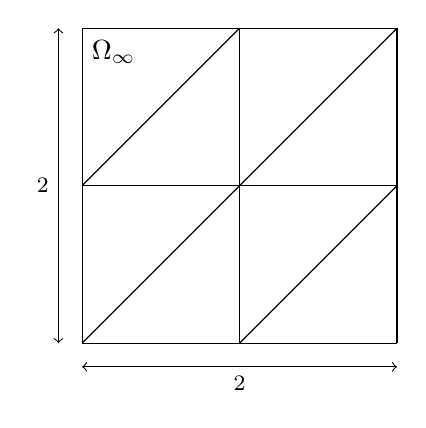
\begin{tikzpicture} [dot/.style={draw,rectangle,minimum size=4mm,inner sep=0pt,outer sep=0pt,thick}, step=2cm]
		\draw [thin] (0,0) grid (4,4);
		\draw [thin] (0,2) -- (2,4);
		\draw [thin] (0,0) -- (4,4);
		\draw [thin] (2,0) -- (4,2);
		\node [font=\normalsize] at (0.4,3.7) {$\Omega_\infty$};
	% \begin{tikzpicture} [dot/.style={draw,rectangle,minimum size=4mm,inner sep=0pt,outer sep=0pt,thick}]
		% \draw [thin] (0,0) grid (4,4);
		% \draw [thin] (0,3) -- (1,4);
		% \draw [thin] (0,2) -- (2,4);
		% \draw [thin] (0,1) -- (3,4);
		% \draw [thin] (0,0) -- (4,4);
		% \draw [thin] (1,0) -- (4,3);
		% \draw [thin] (2,0) -- (4,2);
		% \draw [thin] (3,0) -- (4,1);
		% \node [font=\normalsize] at (0.35,3.75) {$\Omega_\infty$};
		\draw [thin,<->] (0,-0.3) -- (4,-0.3) node[draw=none,fill=none,font=\footnotesize,midway,below] {2};
		\draw [thin,<->] (-0.3,0) -- (-0.3,4) node[draw=none,fill=none,font=\footnotesize,midway,left] {2};
	\end{tikzpicture}
%	\qquad\qquad
%	\begin{tikzpicture}
%		\draw[thin] (2,2) circle (2 cm);
%		\draw[thin] (1.29289321882,1.29289321882) -- (1.29289321882,2.70710678118);
%		\draw[thin] (1.29289321882,1.29289321882) -- (2.70710678118,1.29289321882);
%		\draw[thin] (2.70710678118,2.70710678118) -- (2.70710678118,1.29289321882);
%		\draw[thin] (2.70710678118,2.70710678118) -- (1.29289321882,2.70710678118);
%		\draw[thin] (0.58578643763,0.58578643763) -- (1.29289321882,1.29289321882);
%		\draw[thin] (3.41421356236,3.41421356236) -- (2.70710678118,2.70710678118);
%		\draw[thin] (3.41421356236,0.58578643763) -- (2.70710678118,1.29289321882);
%		\draw[thin] (0.58578643763,3.41421356236) -- (1.29289321882,2.70710678118);
%		% \node at (2,2) {\includegraphics[clip=true, trim = 0.5cm 0 0.5cm 4cm, width=0.4\textwidth]{Figures/Obstacle_mesh.png}};
%		\draw [thin,<->] (0,-0.3) -- (4,-0.3) node[draw=none,fill=none,font=\footnotesize,midway,below] {2};
%		\node [font=\normalsize] at (0.4,3.7) {$\Omega_2$};
%    \end{tikzpicture}
	\caption{\label{fig:ObstacleMesh} Initial FE meshes for domain $\Omega_\infty$ mesh sizes $h = h_\infty$, respectively. (l): Initial triangular mesh for $(\mathbb{P}_p\text{-bubble},\mathbb{P}_{p-1}\text{-broken})$ pair on $\Omega_\infty$. We consider various polynomial orders $p \geq 1$ and mesh sizes.}
\end{figure}
\end{frame}

\begin{frame}\frametitle{Experiment 1}
\begin{center}
{\color{Maroon} \Large How does PG behave over various meshes and polynomials orders?}
\end{center}
\end{frame}

\begin{frame}\frametitle{Experiment 1}
\begin{itemize}
\item Set $g=u$, where $u(x,y)$ is the smooth manufactured solution
\begin{equation}
\label{eq:Biactivity_SmoothManufacturedSolution}
	u(x,y)
	=
	\begin{cases}
		0 & \text{if~} x < 0\,,\\
		x^4 & \text{otherwise,}\\
	\end{cases}
	\quad
	% \iff
	\text{implied by}
	% \impliedby
	\quad
	f(x,y)
	=
	\begin{cases}
		0 & \text{if~} x < 0\,,\\
		-12x^2 & \text{otherwise.}\\
	\end{cases}
\end{equation}
\item $\lambda \equiv 0$:  this is a \textbf{biactive} solution, meaning
problem is nonsmooth at the solution.
%\item The active/contact set has positive Lebesgue measure.
\item Proximal point is a (slow) fixed point method if $\alpha$ is left fixed. We choose: 
\begin{equation}
\label{eq:ObstacleStepSizes_superexponential}
	\alpha_1 = 1\,,
	\quad
	\alpha_k
	=
	\min\bigl\{ \max\bigl\{\alpha_1,r^{q^{k-1}} - \alpha_{k-1}\bigr\} , 10^{10} \bigr\}
	\,,
	\quad
	k = 2,3,\ldots,
\end{equation}
where $r = q = 1.5$.  
\item Once $\alpha_k = 10^{10}$, we can check successive iterates as a stopping criterion.
\end{itemize}
\end{frame}

\begin{frame}\frametitle{Experiment 1: Results}

\begin{table}
\centering
\tiny
\renewcommand{\arraystretch}{1.3}
\begin{tabular}{ |c|c|c|c|c|c|c| }
 \hhline{|>{\arrayrulecolor{white}}-->{\arrayrulecolor{black}}|-----|}
 \multicolumn{2}{c|}{} & \multicolumn{5}{c|}{\cellcolor{lightgray!15} \small\raisebox{5pt}{\vphantom{f}} Progress of the iterates $\|u_h^{k} - u_h^{k-1}\|_{H^1(\Omega_\infty)}$ for various $h$ and $p$}\\[3pt]
 \hhline{|>{\arrayrulecolor{white}}-->{\arrayrulecolor{black}}|-----|}
 \multicolumn{2}{c|}{}& \multicolumn{3}{c|}{\cellcolor{lightgray!05} Polynomial order $p = 1$} & \multicolumn{2}{c|}{\cellcolor{lightgray!10} Polynomial order $p = 2$}\\
 \hline
 \rowcolor{lightgray!15}
 $k$ & $\alpha_{k}$ & $h_\infty/16$ & $h_\infty/32$ & $h_\infty/64$ & $h_\infty/16$ & $h_\infty/32$ \\
 \hline
\cellcolor{lightgray!05}   1 & \cellcolor{lightgray!01}   $1.0$              & $2.10\cdot 10^{0}$   & $2.10\cdot 10^{0}$   & $2.10\cdot 10^{0}$   & $2.10\cdot 10^{0}$   & $2.10\cdot 10^{0}$   \\
\cellcolor{lightgray!05}   2 & \cellcolor{lightgray!01}   $1.0$              & $6.45\cdot 10^{-1}$  & $6.45\cdot 10^{-1}$  & $6.45\cdot 10^{-1}$  & $6.45\cdot 10^{-1}$  & $6.45\cdot 10^{-1}$  \\
\cellcolor{lightgray!05}   3 & \cellcolor{lightgray!01}   $1.49$             & $1.73\cdot 10^{-1}$  & $1.73\cdot 10^{-1}$  & $1.73\cdot 10^{-1}$  & $1.73\cdot 10^{-1}$  & $1.73\cdot 10^{-1}$  \\
\cellcolor{lightgray!05}   4 & \cellcolor{lightgray!01}   $2.43$             & $1.10\cdot 10^{-1}$  & $1.10\cdot 10^{-1}$  & $1.10\cdot 10^{-1}$  & $1.10\cdot 10^{-1}$  & $1.10\cdot 10^{-1}$  \\
\cellcolor{lightgray!05}   5 & \cellcolor{lightgray!01}   $5.35$             & $7.76\cdot 10^{-2}$  & $7.77\cdot 10^{-2}$  & $7.77\cdot 10^{-2}$  & $7.77\cdot 10^{-2}$  & $7.77\cdot 10^{-2}$  \\
\cellcolor{lightgray!05}   6 & \cellcolor{lightgray!01}   $1.64\cdot 10^{1}$ & $4.76\cdot 10^{-2}$  & $4.77\cdot 10^{-2}$  & $4.77\cdot 10^{-2}$  & $4.77\cdot 10^{-2}$  & $4.77\cdot 10^{-2}$  \\
\cellcolor{lightgray!05}   7 & \cellcolor{lightgray!01}   $8.50\cdot 10^{1}$ & $2.24\cdot 10^{-2}$  & $2.25\cdot 10^{-2}$  & $2.25\cdot 10^{-2}$  & $2.25\cdot 10^{-2}$  & $2.25\cdot 10^{-2}$  \\
\cellcolor{lightgray!05}   8 & \cellcolor{lightgray!01}   $9.35\cdot 10^{2}$ & $5.82\cdot 10^{-3}$  & $5.84\cdot 10^{-3}$  & $5.85\cdot 10^{-3}$  & $5.85\cdot 10^{-3}$  & $5.85\cdot 10^{-3}$  \\
\cellcolor{lightgray!05}   9 & \cellcolor{lightgray!01}   $3.17\cdot 10^{4}$ & $6.04\cdot 10^{-4}$  & $6.07\cdot 10^{-4}$  & $6.07\cdot 10^{-4}$  & $6.07\cdot 10^{-4}$  & $6.07\cdot 10^{-4}$  \\
\cellcolor{lightgray!05}  10 & \cellcolor{lightgray!01}   $5.85\cdot 10^{6}$ & $1.80\cdot 10^{-5}$  & $1.81\cdot 10^{-5}$  & $1.81\cdot 10^{-5}$  & $1.81\cdot 10^{-5}$  & $1.81\cdot 10^{-5}$  \\
\cellcolor{lightgray!05}  11 & \cellcolor{lightgray!01}   $1\cdot 10^{10}$   & $9.41\cdot 10^{-8}$  & $9.47\cdot 10^{-8}$  & $9.49\cdot 10^{-8}$  & $9.50\cdot 10^{-8}$  & $9.50\cdot 10^{-8}$  \\
\cellcolor{lightgray!05}  12 & \cellcolor{lightgray!01}   $1\cdot 10^{10}$   & $2.10\cdot 10^{-12}$ & $2.00\cdot 10^{-12}$ & $1.96\cdot 10^{-12}$ & $1.92\cdot 10^{-12}$ & $1.95\cdot 10^{-10}$ \\
 \hline
 \rowcolor{lightgray!05}
 \multicolumn{2}{|c|}{\cellcolor{lightgray!15} Tot. linear solves} & $21$ & $20$ & $19$ & $19$ & $19$ \\
 \hline
\end{tabular}
%\caption{\label{tab:BiactivityMeshIndependence}
%Biactivity.
%Table of increments $\|u_h^{k} - u_h^{k-1}\|_{H^1(\Omega_\infty)}$ for various mesh sizes $h$ and polynomial orders $p$ using the triangular element $(\mathbb{P}_p\text{-bubble},\mathbb{P}_{p-1}\text{-broken})$ discretization.
%% of the biactive manufactured solution~\cref{eq:Biactivity_SmoothManufacturedSolution} on $\Omega = \Omega_\infty$.
%The initial degrees of freedom for $u_h$ and $\psi_h$ were set to zero at the beginning of each run.
%Between eight and ten Newton iterations performed by the PETSc Newton solver used for each initial subproblem solve and then only one Newton solve was used for each of the following subproblems.
%The convergence of the increments for each fixed $k$ and the boundedness of the number of linear solves indicates \emph{mesh-independence}.
%}
\end{table}
\end{frame}

\begin{frame}\frametitle{Experiment 1: Results}
\begin{figure}
	\centering
	\begin{tikzpicture}
		\node at (-3.35,0.5) {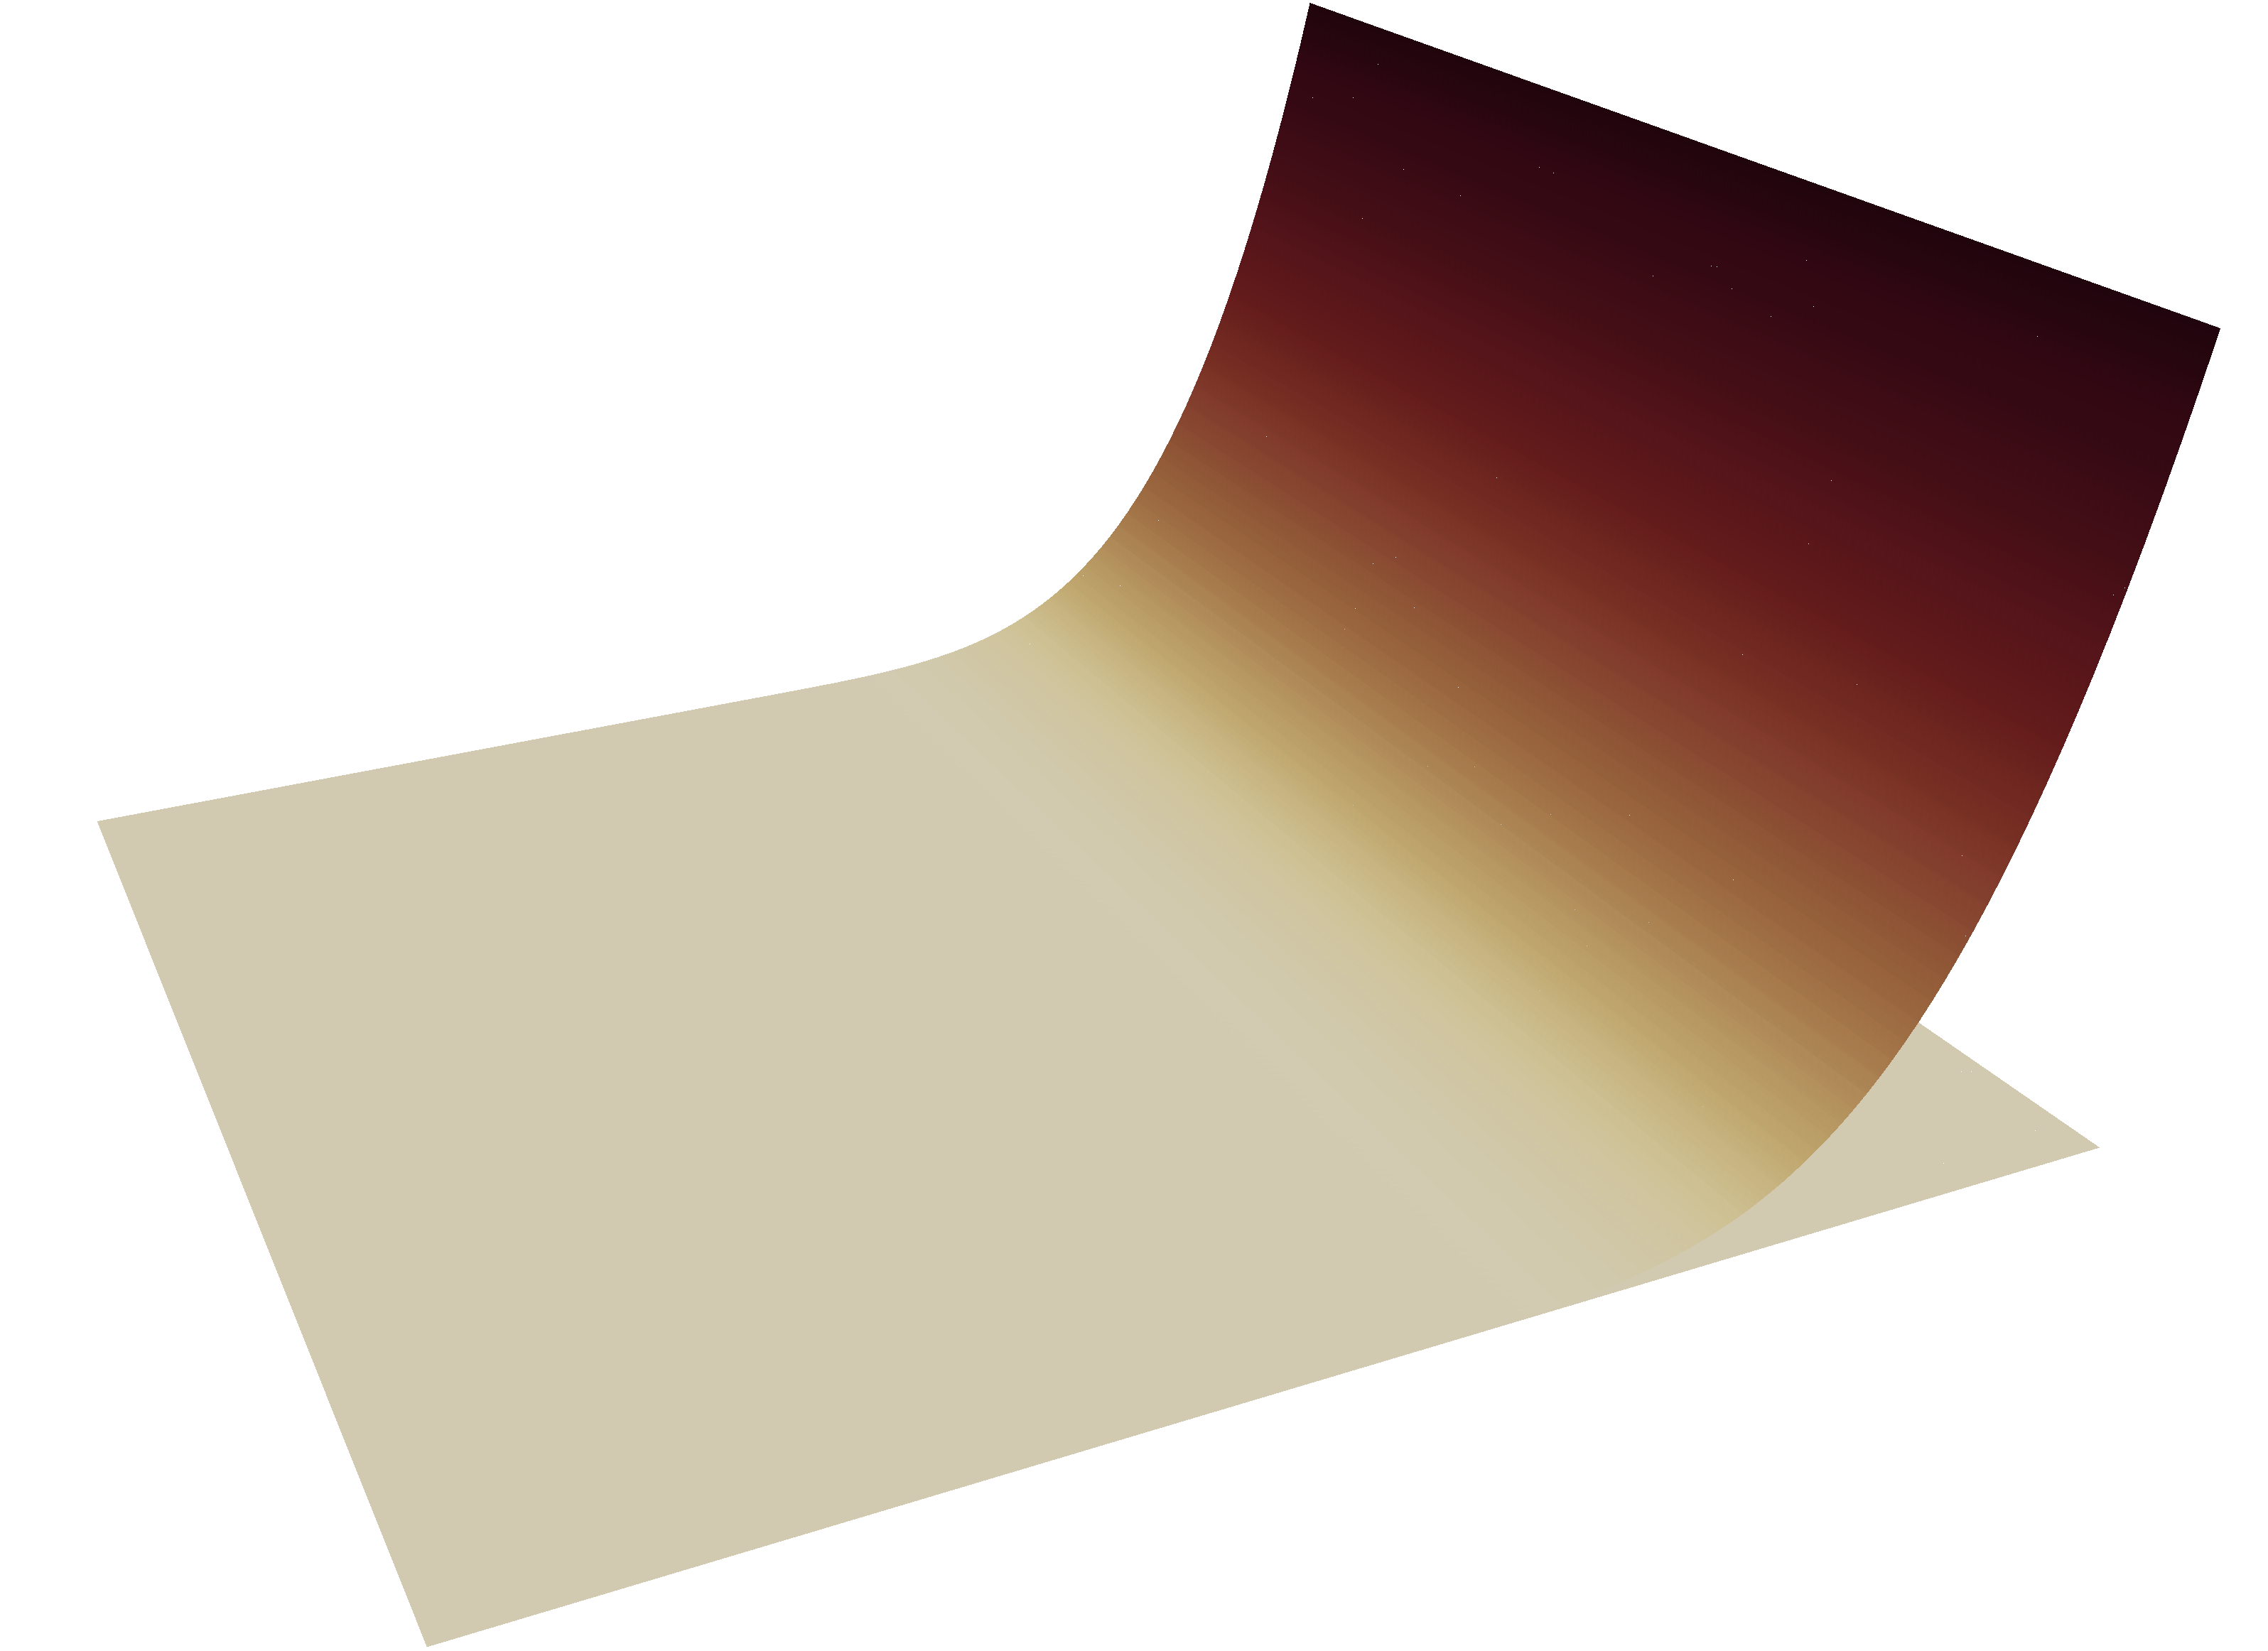
\includegraphics[height=1.5in]{Figures/ObstacleExperiment1.png}};
		\node at (3.25,0.4) {
			   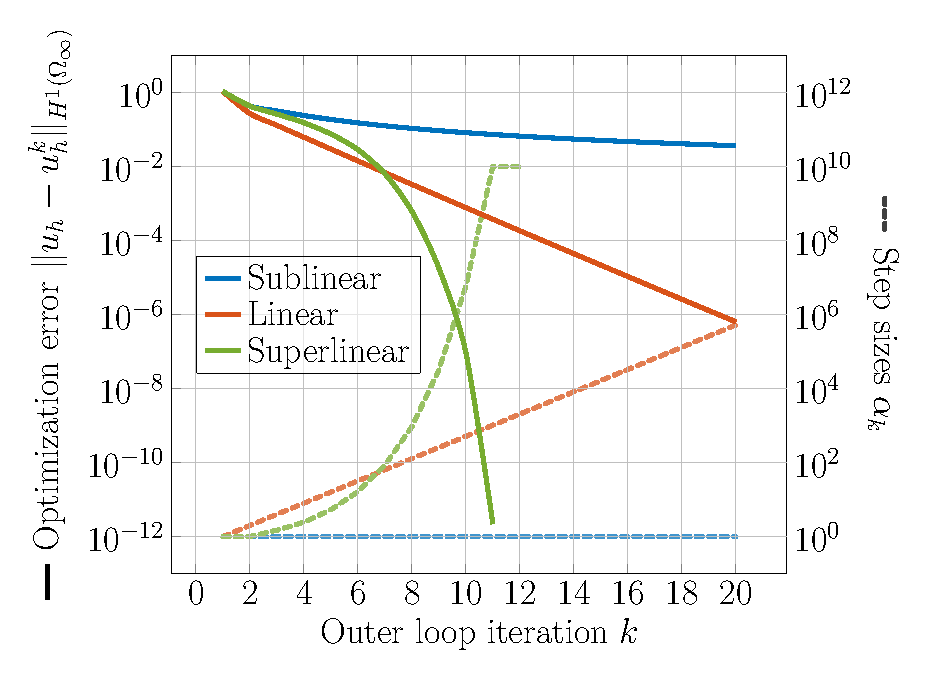
\includegraphics[clip=true, trim= 0 0 0.35cm 0, height=2.1in]{Figures/tikz/FEniCS_plots/example0/example0_ConvergenceRate.pdf}
		};
	    \node at (-0.5,0.4) {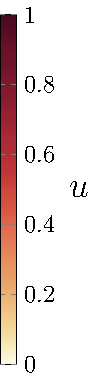
\includegraphics[height=2cm]{Figures/tikz/FEniCS_plots/example0/colorbar/colorbar0.pdf}};
	    \node at (-2.2,-1.35) {\scriptsize $
	    	u(x,y)
	    	=
	    	\begin{cases}
	    		0 & \text{if~} x < 0\\
	    		x^4 & \text{otherwise}\\
	    	\end{cases}
	    $};
    \end{tikzpicture}
%	\caption{
%	\label{fig:BiactiveIterationComplexity}
%	Biactivity.
%	Verifying the convergence orders predicted by \Cref{cor:ConvergenceRates} with the $(\mathbb{P}_1\text{-bubble},\mathbb{P}_{0}\text{-broken})$ discretization (FEniCSx).
%	Left: The exact solution.
%	Right: Plots of the optimization error $\|u_h - u_h^k\|_{H^1(\Omega_\infty)}$ and corresponding step size $\alpha_k$ when $h = h_\infty / 16$.
%	The blue curve tracks the \emph{sublinear} convergence induced by the fixed step size rule $\alpha_k = 1$.
%	Meanwhile, the step size rules \cref{eq:ObstacleStepSizes_geometric} and \cref{eq:ObstacleStepSizes_superexponential} induce \emph{linear} (red) and \emph{superlinear} (green) convergence, respectively.
%	The results are similar on finer meshes due to mesh-independence; cf.~\Cref{tab:BiactivityMeshIndependence}.
%	}
\end{figure}
\end{frame}

\begin{frame}\frametitle{Experiment 2}
\begin{center}
{\color{Maroon} \Large How does PG on optimality conditions and strict complementarity?}
\end{center}
\end{frame}

\begin{frame}\frametitle{Experiment 2}
\begin{itemize}
\item In this experiment, we set $g = 0$ and define 
\begin{equation}
\label{eq:StrictComplementarity_RHS}
	f(x,y)
	=
	2 \pi^2 \sin(\pi x)\sin(\pi y)
	\,.
\end{equation}
%See~\Cref{fig:StrictComplementarityConvergenceOrder} for a fine mesh ($h = h_\infty/128$) solution $u_h$ and Lagrange multiplier $\lambda_h$.
\item We aim to check convergence of the discrete solution via the KKT conditions:
%This is useful to assess \textit{a posteriori} the optimality of the discrete solution when the true solution is unknown.
%To this end, we consider the complementarity condition:
 \[
 \aligned
 \big|\int_{\Omega} \lambda u \dd x\big| &= 0, \text{ complementary slackness, }\\
 \int_{\Omega} \max\{-u,0\} \dd x &= 0, \text{ primal feasibility, }\\
 \int_{\Omega} \max\{-\lambda,0\} \dd x &= 0, \text{ dual feasibility.}
 \endaligned
 \]
% \item 
%We note that the discrete solution $\tilde{u}_h = \exp\psi_h$ is always feasible by construction, i.e., $\tilde{u}_h \geq 0$.
%Therefore, in order to glean more interesting information about the proximal Galerkin solution, we focus on discrete versions of the KKT conditions formulated in terms of the solution variable $u_h$.
%The discrete KKT conditions that we checked are recorded in \Cref{tab:KKT}.
%From the results in this table, we see that discrete primal feasibility, $\int_{\Omega} \max\{-u_h,0\} \dd x = 0$, is achieved only in the limit $h \to 0$.
%However, discrete complementarity, $\big|\int_{\Omega} \lambda_h u_h \dd x\big| = 0$, and discrete dual feasibility, $\int_{\Omega} \max\{-\lambda_h,0\} \dd x = 0$, appear to hold for all mesh sizes.
% at least up to round-off errors.
%The results of this experiment can be reproduced by running the FEniCSx code \texttt{obstacle.py} available at \cite{ZenodoCode}.

\end{itemize}
\end{frame}

\begin{frame}\frametitle{Experiment 2: Results}
\begin{table}
\centering
\small
\renewcommand{\arraystretch}{1.3}
\begin{tabular}{ |c|c|c|c| }
 \hline
 \rowcolor{lightgray!10}
  &&&
  \\
 \rowcolor{lightgray!10}
  \multirow{-2}{*}{$h$} & \multirow{-2}{3cm}{\centering {\small Complementarity} $\big|\int_{\Omega_\infty} \lambda_h u_h \dd x\big|$} & \multirow{-2}{3cm}{\centering {\small Primal feasibility} $\int_{\Omega_\infty} \max\{-u_h,0\} \dd x$} & \multirow{-2}{3cm}{\centering {\small Dual feasibility} $\int_{\Omega_\infty} \max\{-\lambda_h,0\} \dd x$}\\
 $h_\infty$     & \multirow{6}{*}{($\text{all less than~} 10^{-14}$)} & $6.97 \cdot 10^{-3}$ & \multirow{6}{*}{($\text{all less than~} 10^{-12}$)} \\
 $h_\infty/2$   &  & $9.09 \cdot 10^{-3}$ & \\
 $h_\infty/4$   &  & $1.16 \cdot 10^{-3}$ & \\
 $h_\infty/8$   &  & $1.69 \cdot 10^{-4}$ & \\
 $h_\infty/16$  &  & $4.08 \cdot 10^{-5}$ & \\
 $h_\infty/32$  &  & $4.53 \cdot 10^{-6}$ & \\
 \hline
\end{tabular}
%\caption{\label{tab:KKT}
%	Strict complementarity.
%	Checking the discrete KKT conditions for the proximal Galerkin solution owing to~\cref{eq:StrictComplementarity_RHS}.
%	Here, we see that primal feasibility is achieved in the limit $h\to 0$.
%	Meanwhile, complementary and dual feasibility holds on all meshes.
%}
\end{table}
%\begin{center}
%Don't forget:  the discrete latent solution $\tilde{u}_h = \exp\psi_h$ is always feasible by construction, i.e., $\tilde{u}_h \geq 0.
%\end{center}
\end{frame}

\begin{frame}\frametitle{Experiment 2: Results}
\begin{figure}
	\centering
	\begin{tikzpicture}
		\node at (-3.35,1) {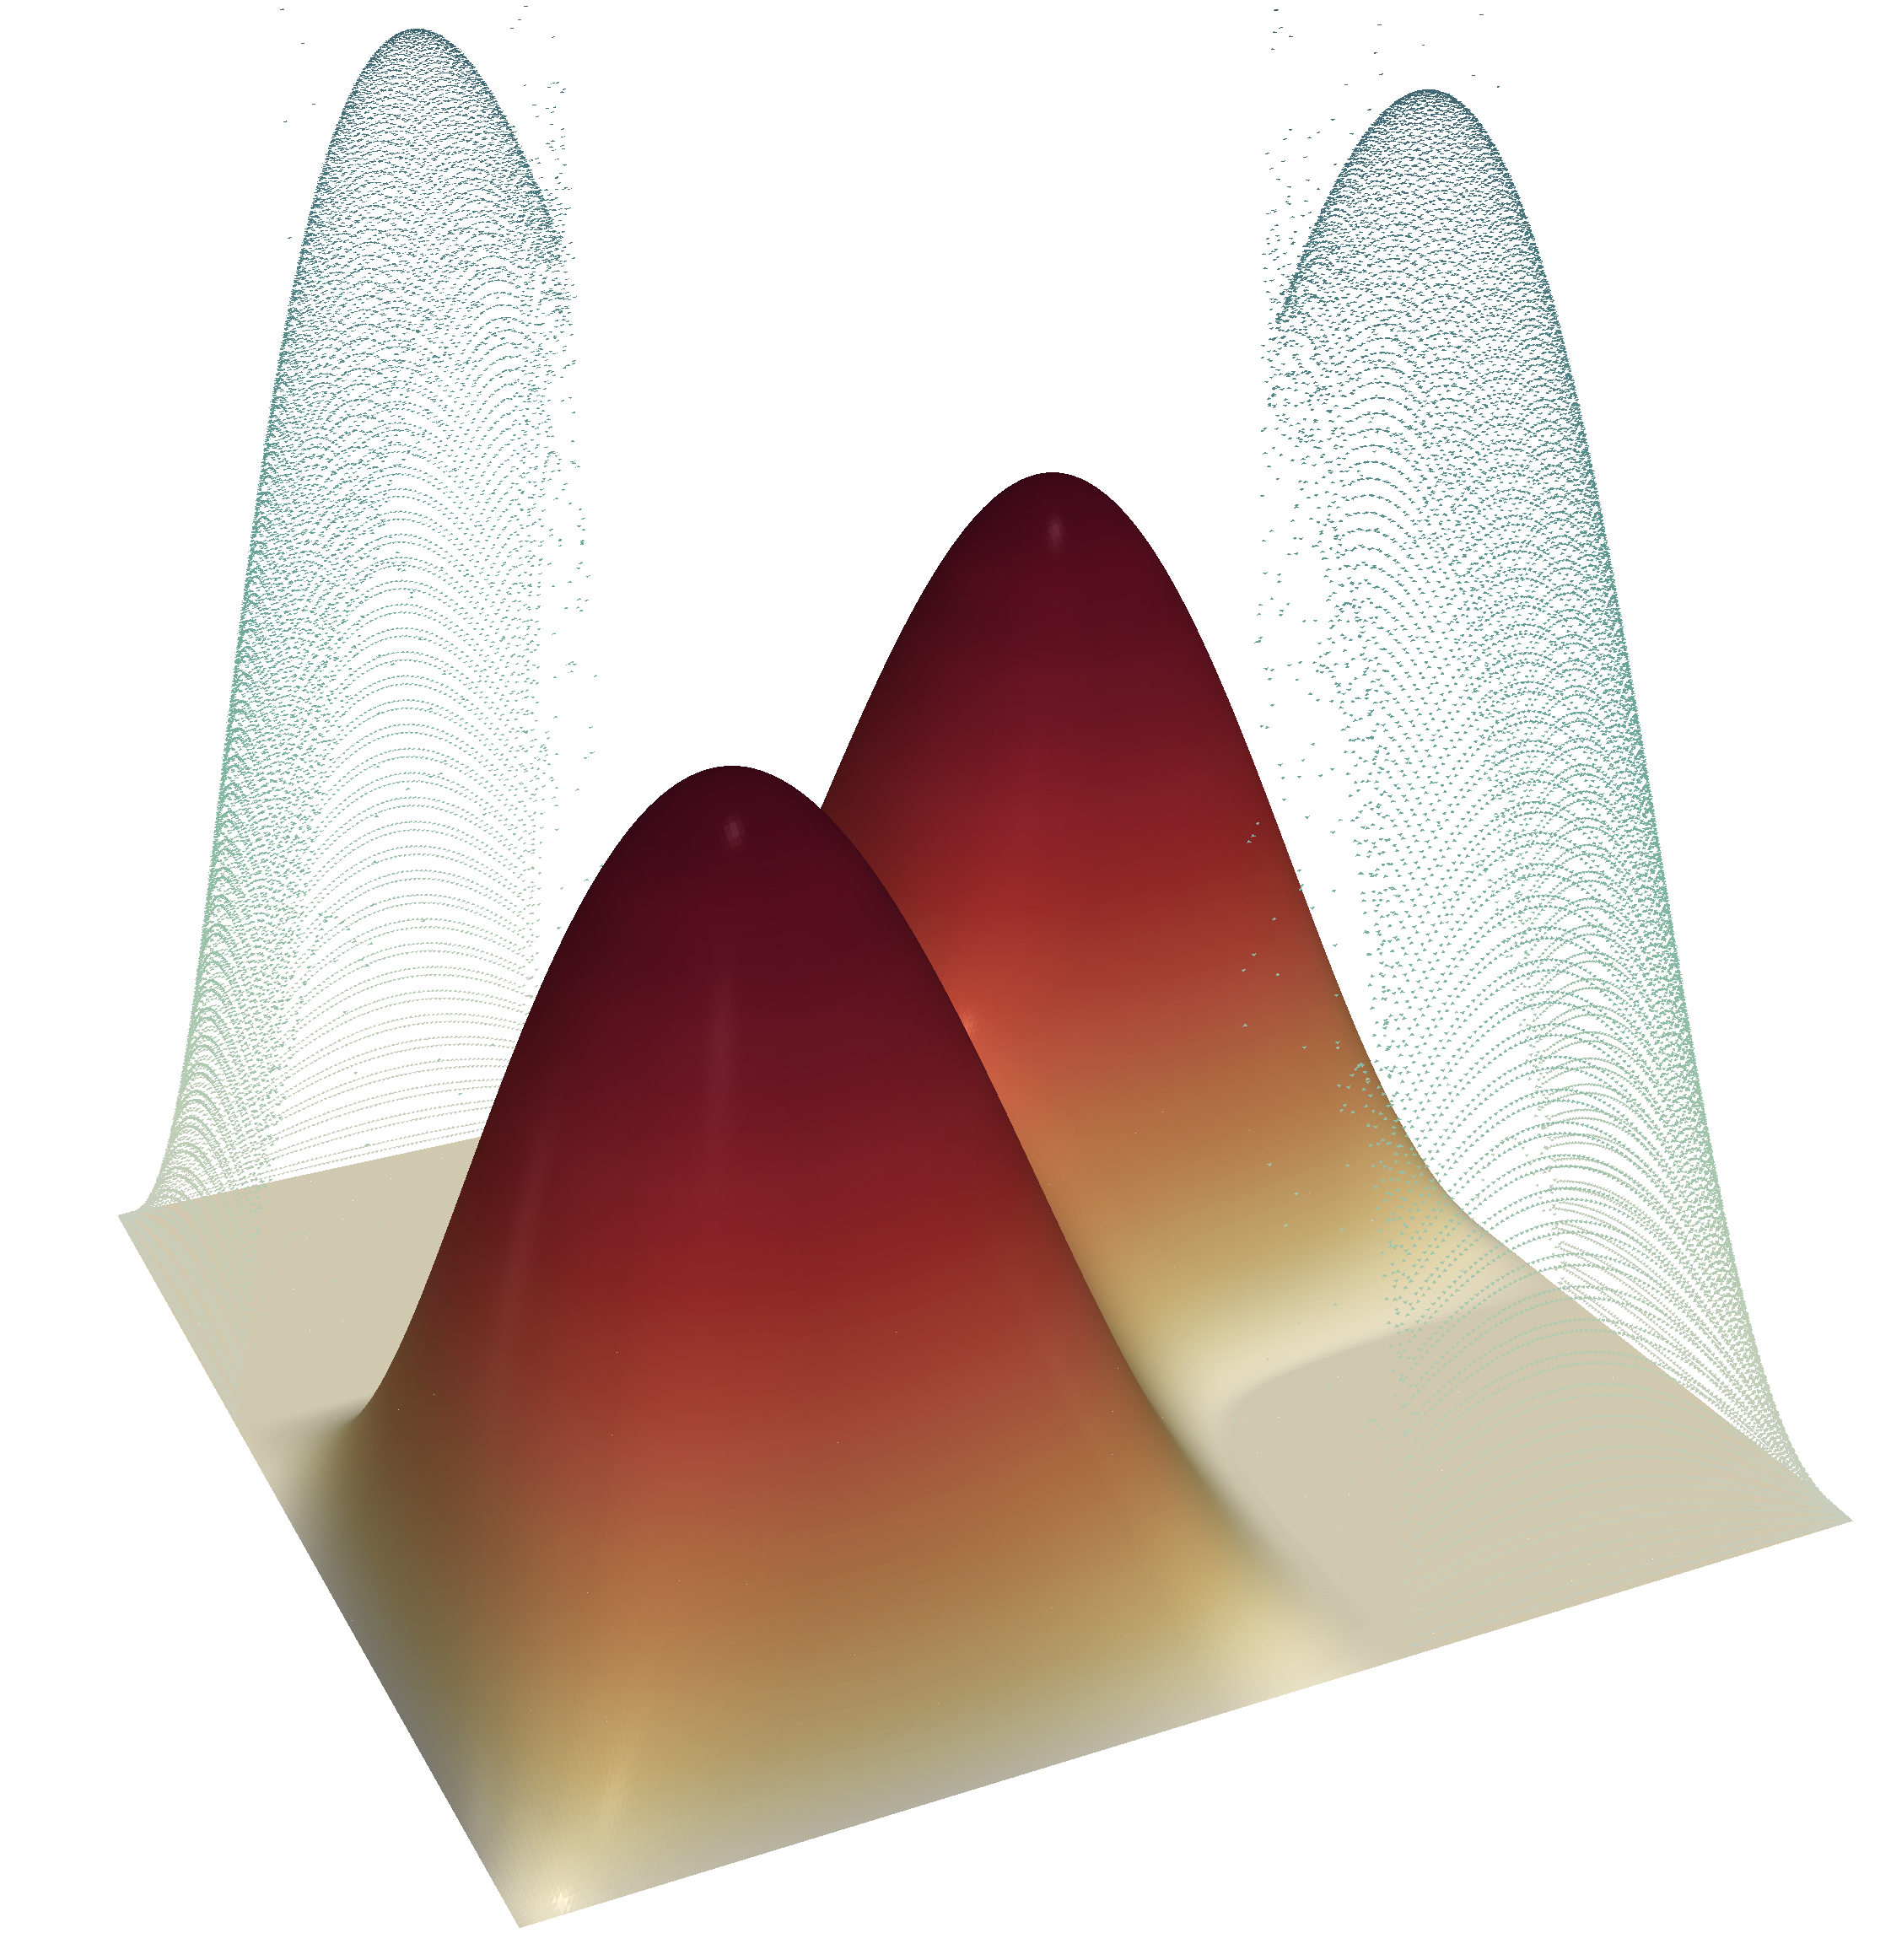
\includegraphics[clip=true, trim= 4cm 0 0 0, height=2.3in]{Figures/ObstacleExperiment2.png}};
		% \node at (-3.35,1) {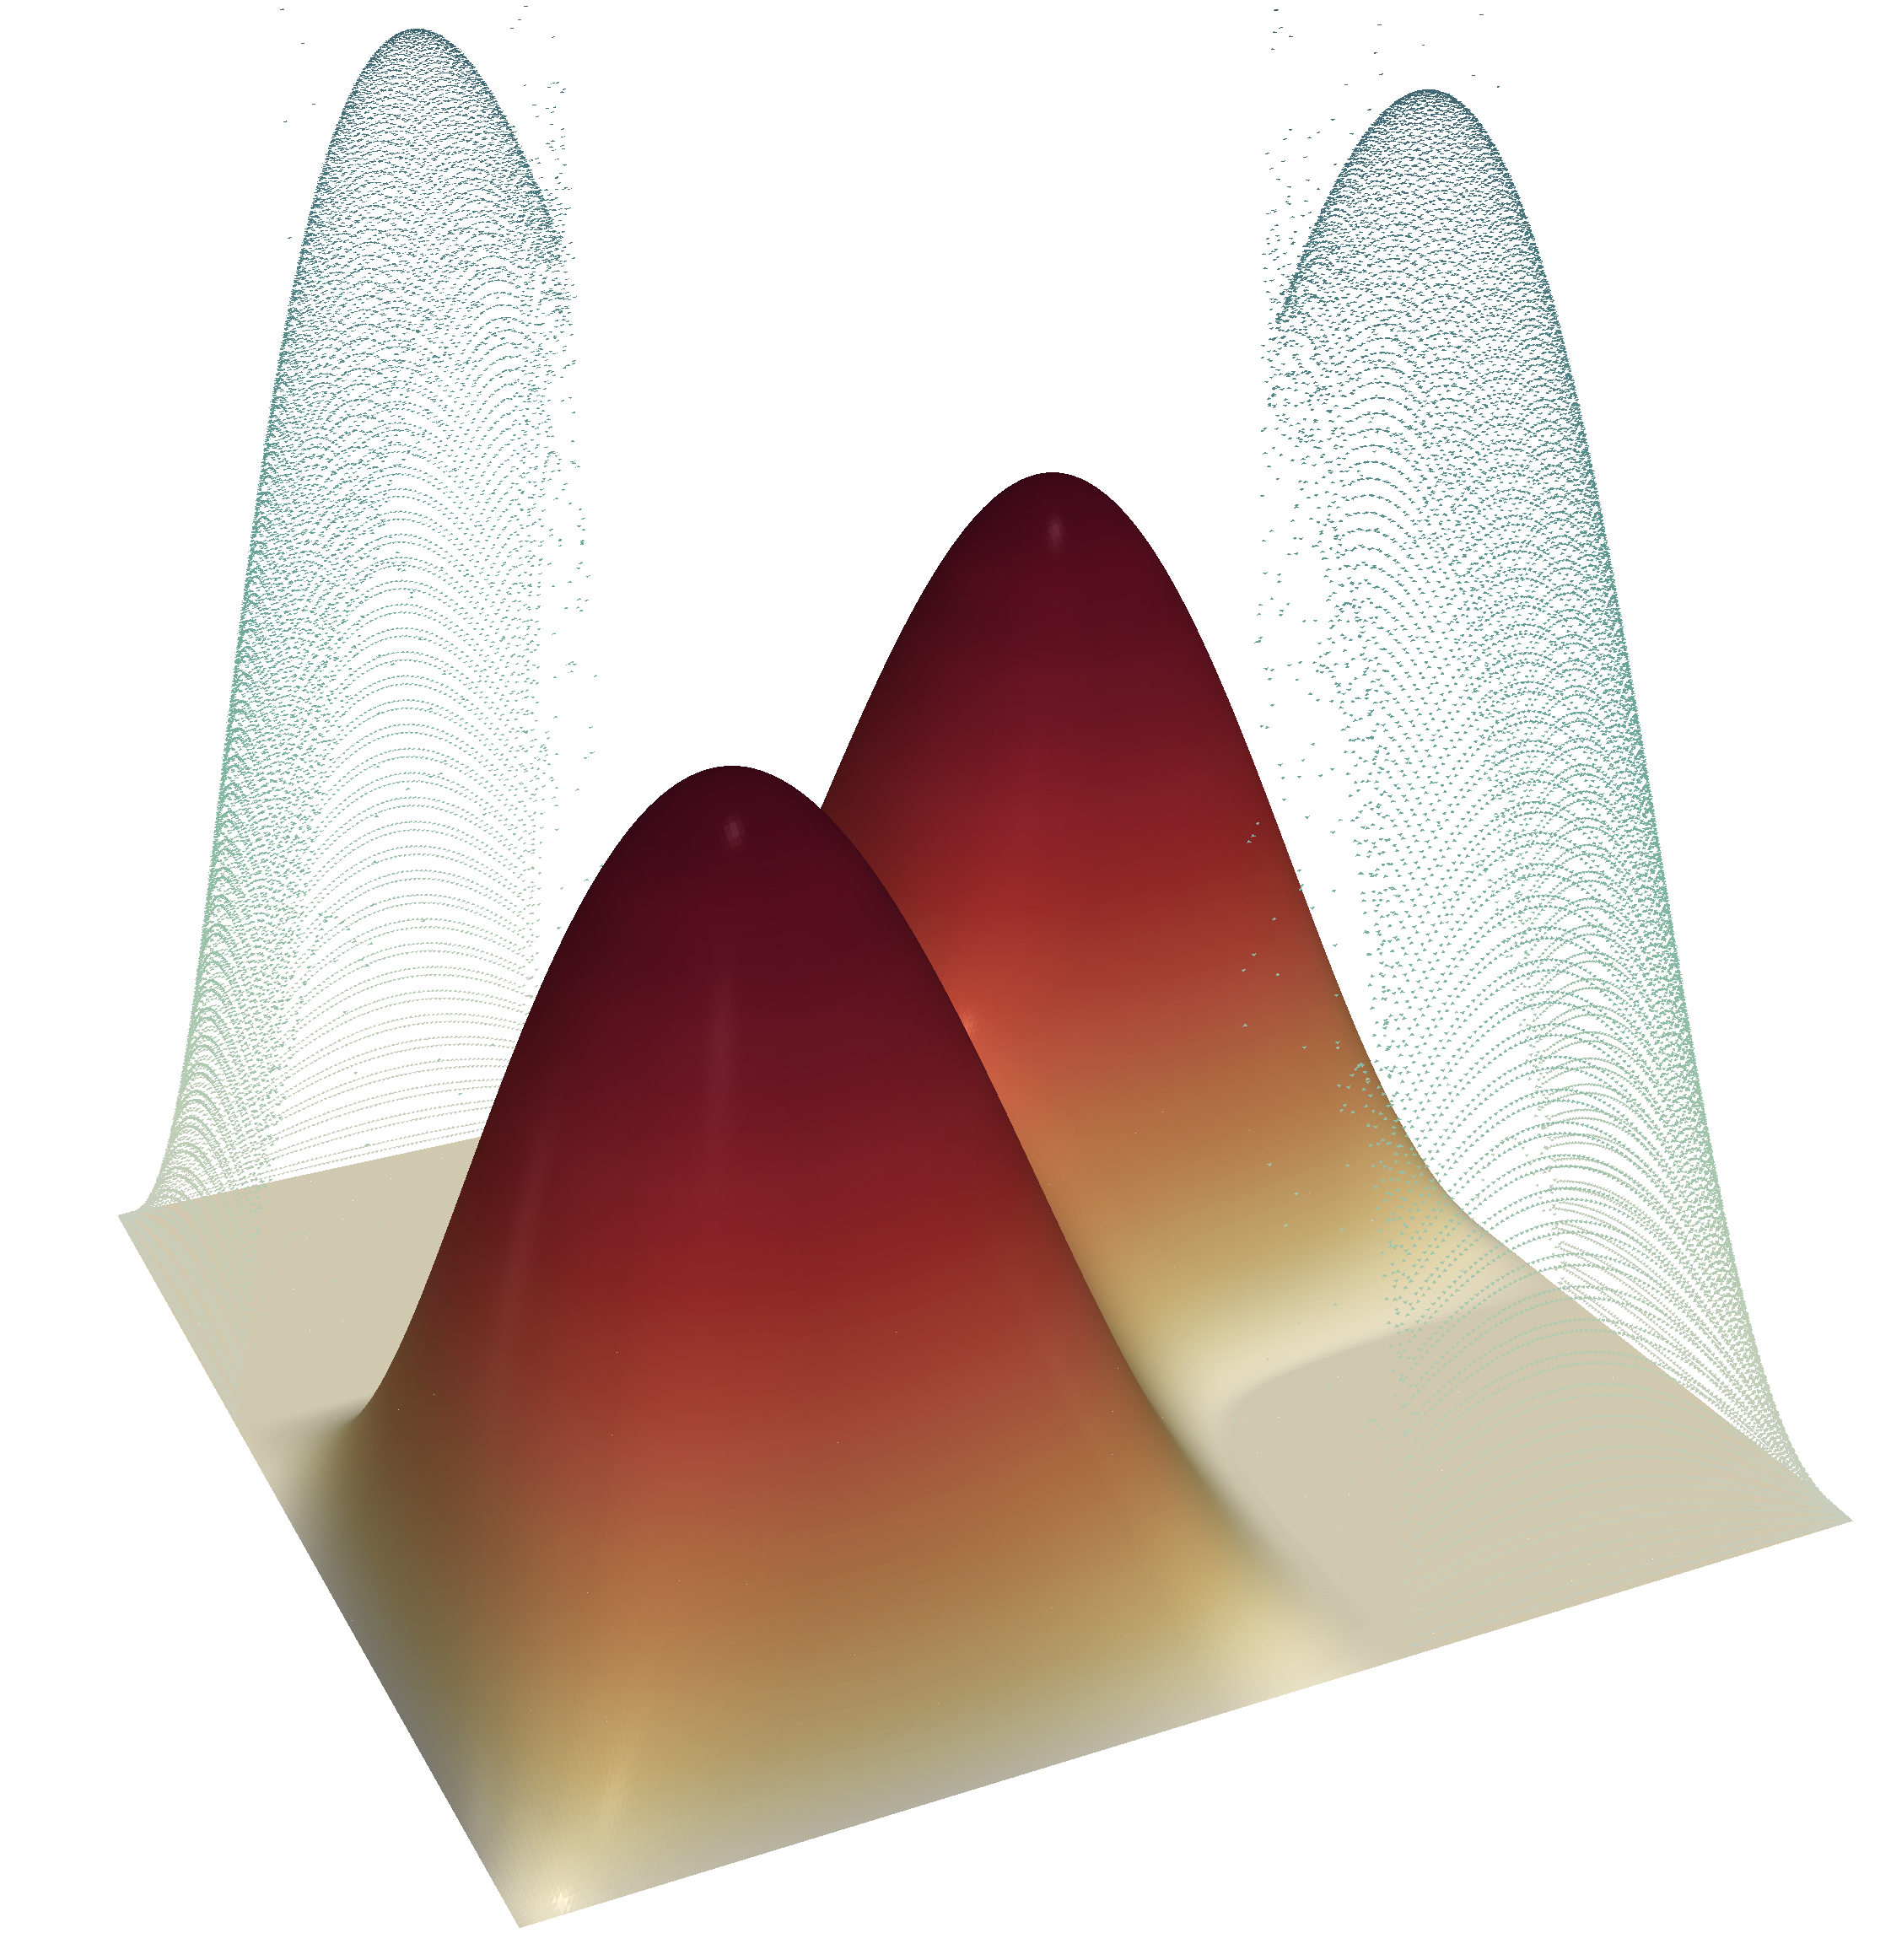
\includegraphics[clip=true, trim= 4cm 0 0 0, width=0.44\textwidth]{Figures/ObstacleExperiment2.png}};
		\node at (3,0.4) {
		   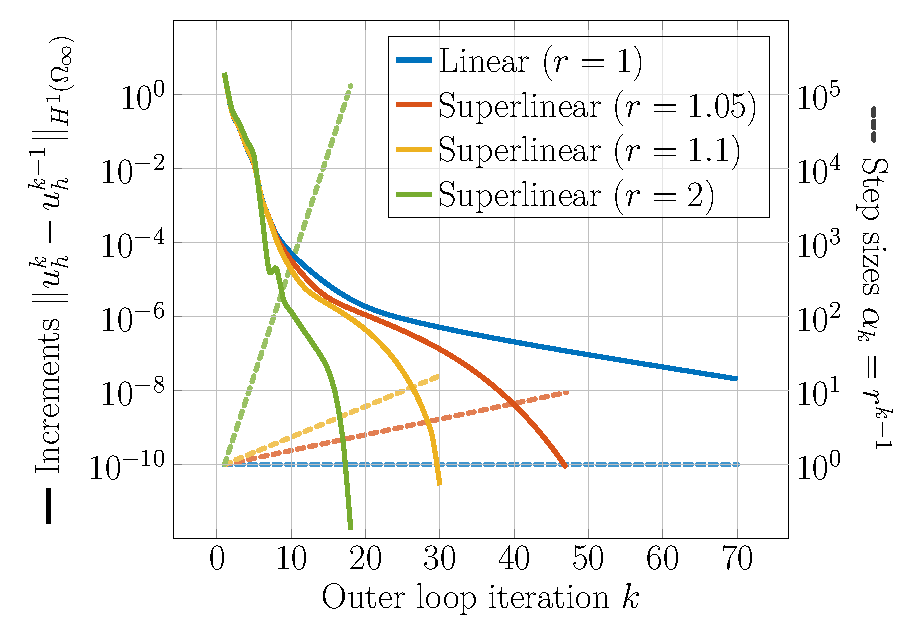
\includegraphics[clip=true, trim= 0 0 0.35cm 0, height=2.1in]{Figures/tikz/FEniCS_plots/example1/example1_ConvergenceRate.pdf}
		};
	    % \node at (-4,2.8) {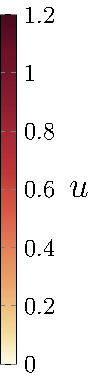
\includegraphics[height=2cm]{Figures/tikz/FEniCS_plots/example1/colorbar/colorbar1.pdf}};
	    \node at (-5.8,-1.2) {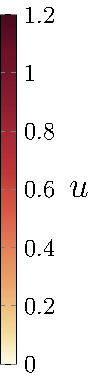
\includegraphics[height=2cm]{Figures/tikz/FEniCS_plots/example1/colorbar/colorbar1.pdf}};
	    \node at (-0.95,2.2) {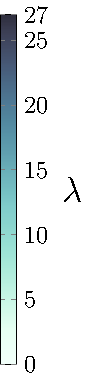
\includegraphics[height=2cm]{Figures/tikz/FEniCS_plots/example1/colorbar/colorbar2.pdf}};
    \end{tikzpicture}
%	\caption{
%	Strict complementarity.
%	Surpassing the convergence orders predicted by \Cref{cor:ConvergenceRates} with the $(\mathbb{P}_1\text{-bubble},\mathbb{P}_{0}\text{-broken})$ discretization (FEniCSx).
%	Left: A high-resolution image of the exact solution $u$ and associated Lagrange multiplier $\lambda$.
%	% corresponding to~\cref{eq:StrictComplementarity_RHS}.
%	Right: Plots of the primal variable increments $\|u_h^{k} - u_h^{k-1}\|_{H^1(\Omega_\infty)}$ and corresponding geometric step sizes $\alpha_k = r^{k-1}$ for mesh size $h = h_\infty / 16$.
%	% The blue curve in demonstrates \emph{linear} convergence coming from the fixed step size rule $\alpha_k = 1$.
%	% Meanwhile, the step size rules \cref{eq:ObstacleStepSizes_geometric} and \cref{eq:ObstacleStepSizes_superexponential} induce \emph{linear} (red) and \emph{superlinear} (green) convergence, respectively.
%	The results are similar on all finer meshes due to mesh-independence; cf.~\Cref{tab:BiactivityMeshIndependence}.
%	Analogous results can also be obtained for higher-order and quadrilateral element discretizations (not shown).
%	\label{fig:StrictComplementarityConvergenceOrder}}
\end{figure}
\end{frame}

\begin{frame}\frametitle{Experiment 3}
\begin{center}
{\color{Maroon} \Large How does PG do with nontrivial obstacles and higher order spaces?}
\end{center}
\end{frame}

\begin{frame}\frametitle{Experiment 3}
\begin{itemize}
\item Set $f = 0$, $g = 0$ and define the obstacle to be the upper surface of a sphere of radius $1/2$, namely
\begin{equation}
\label{eq:SphericalObstacle}
	\phi(x,y) = \sqrt{ 1/4 - x^2 - y^2 }
	\,,
	% ~~
	% \text{if~}
	% \sqrt{x^2 + y^2} \leq 1/2
	% \,,
\end{equation}
if $\sqrt{x^2 + y^2} \leq 1/2$, and assume that $\phi$ is sufficiently negative when $\sqrt{x^2 + y^2} > 1/2$ so that no contact happens on that subdomain.
\item The exact solution on the circular domain $\Omega = \Omega_2$ is found to be
\begin{equation}
	u(x,y) =
	\begin{cases}
		A \ln\sqrt{x^2 + y^2} & \text{if~} \sqrt{x^2 + y^2} > a,\\
		\phi(x,y) & \text{otherwise},\\
	\end{cases}
\end{equation}
where $a = \exp\big(W_{-1}\big(\frac{-1}{2e^2}\big)/2 + 1\big) \approx 0.34898$, $A = {\sqrt{1/4 - a^2}}/{\ln a} \approx -0.34012$, and $W_{j}(\cdot)$ is the $j$-th branch of the Lambert W‐function.
\end{itemize}
\end{frame}

\begin{frame}\frametitle{Experiment 3: Results}
\begin{figure}
	\centering
	\begin{minipage}[c]{0.475\textwidth}
	\small
		\centering
		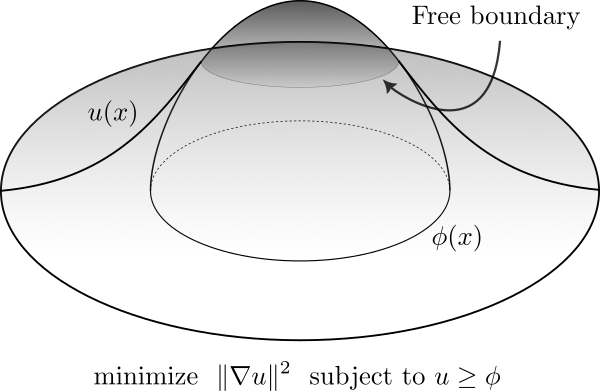
\includegraphics[clip=true, trim= 0 1cm 0 0, height=2cm]{Figures/obstacle_diagram.png}
		\\[0.4em]
		Diagram of problem
	\end{minipage}%,
	\begin{minipage}[c]{0.475\textwidth}
	\small
		\centering
		\begin{minipage}[c]{0.85\textwidth}
		\centering
			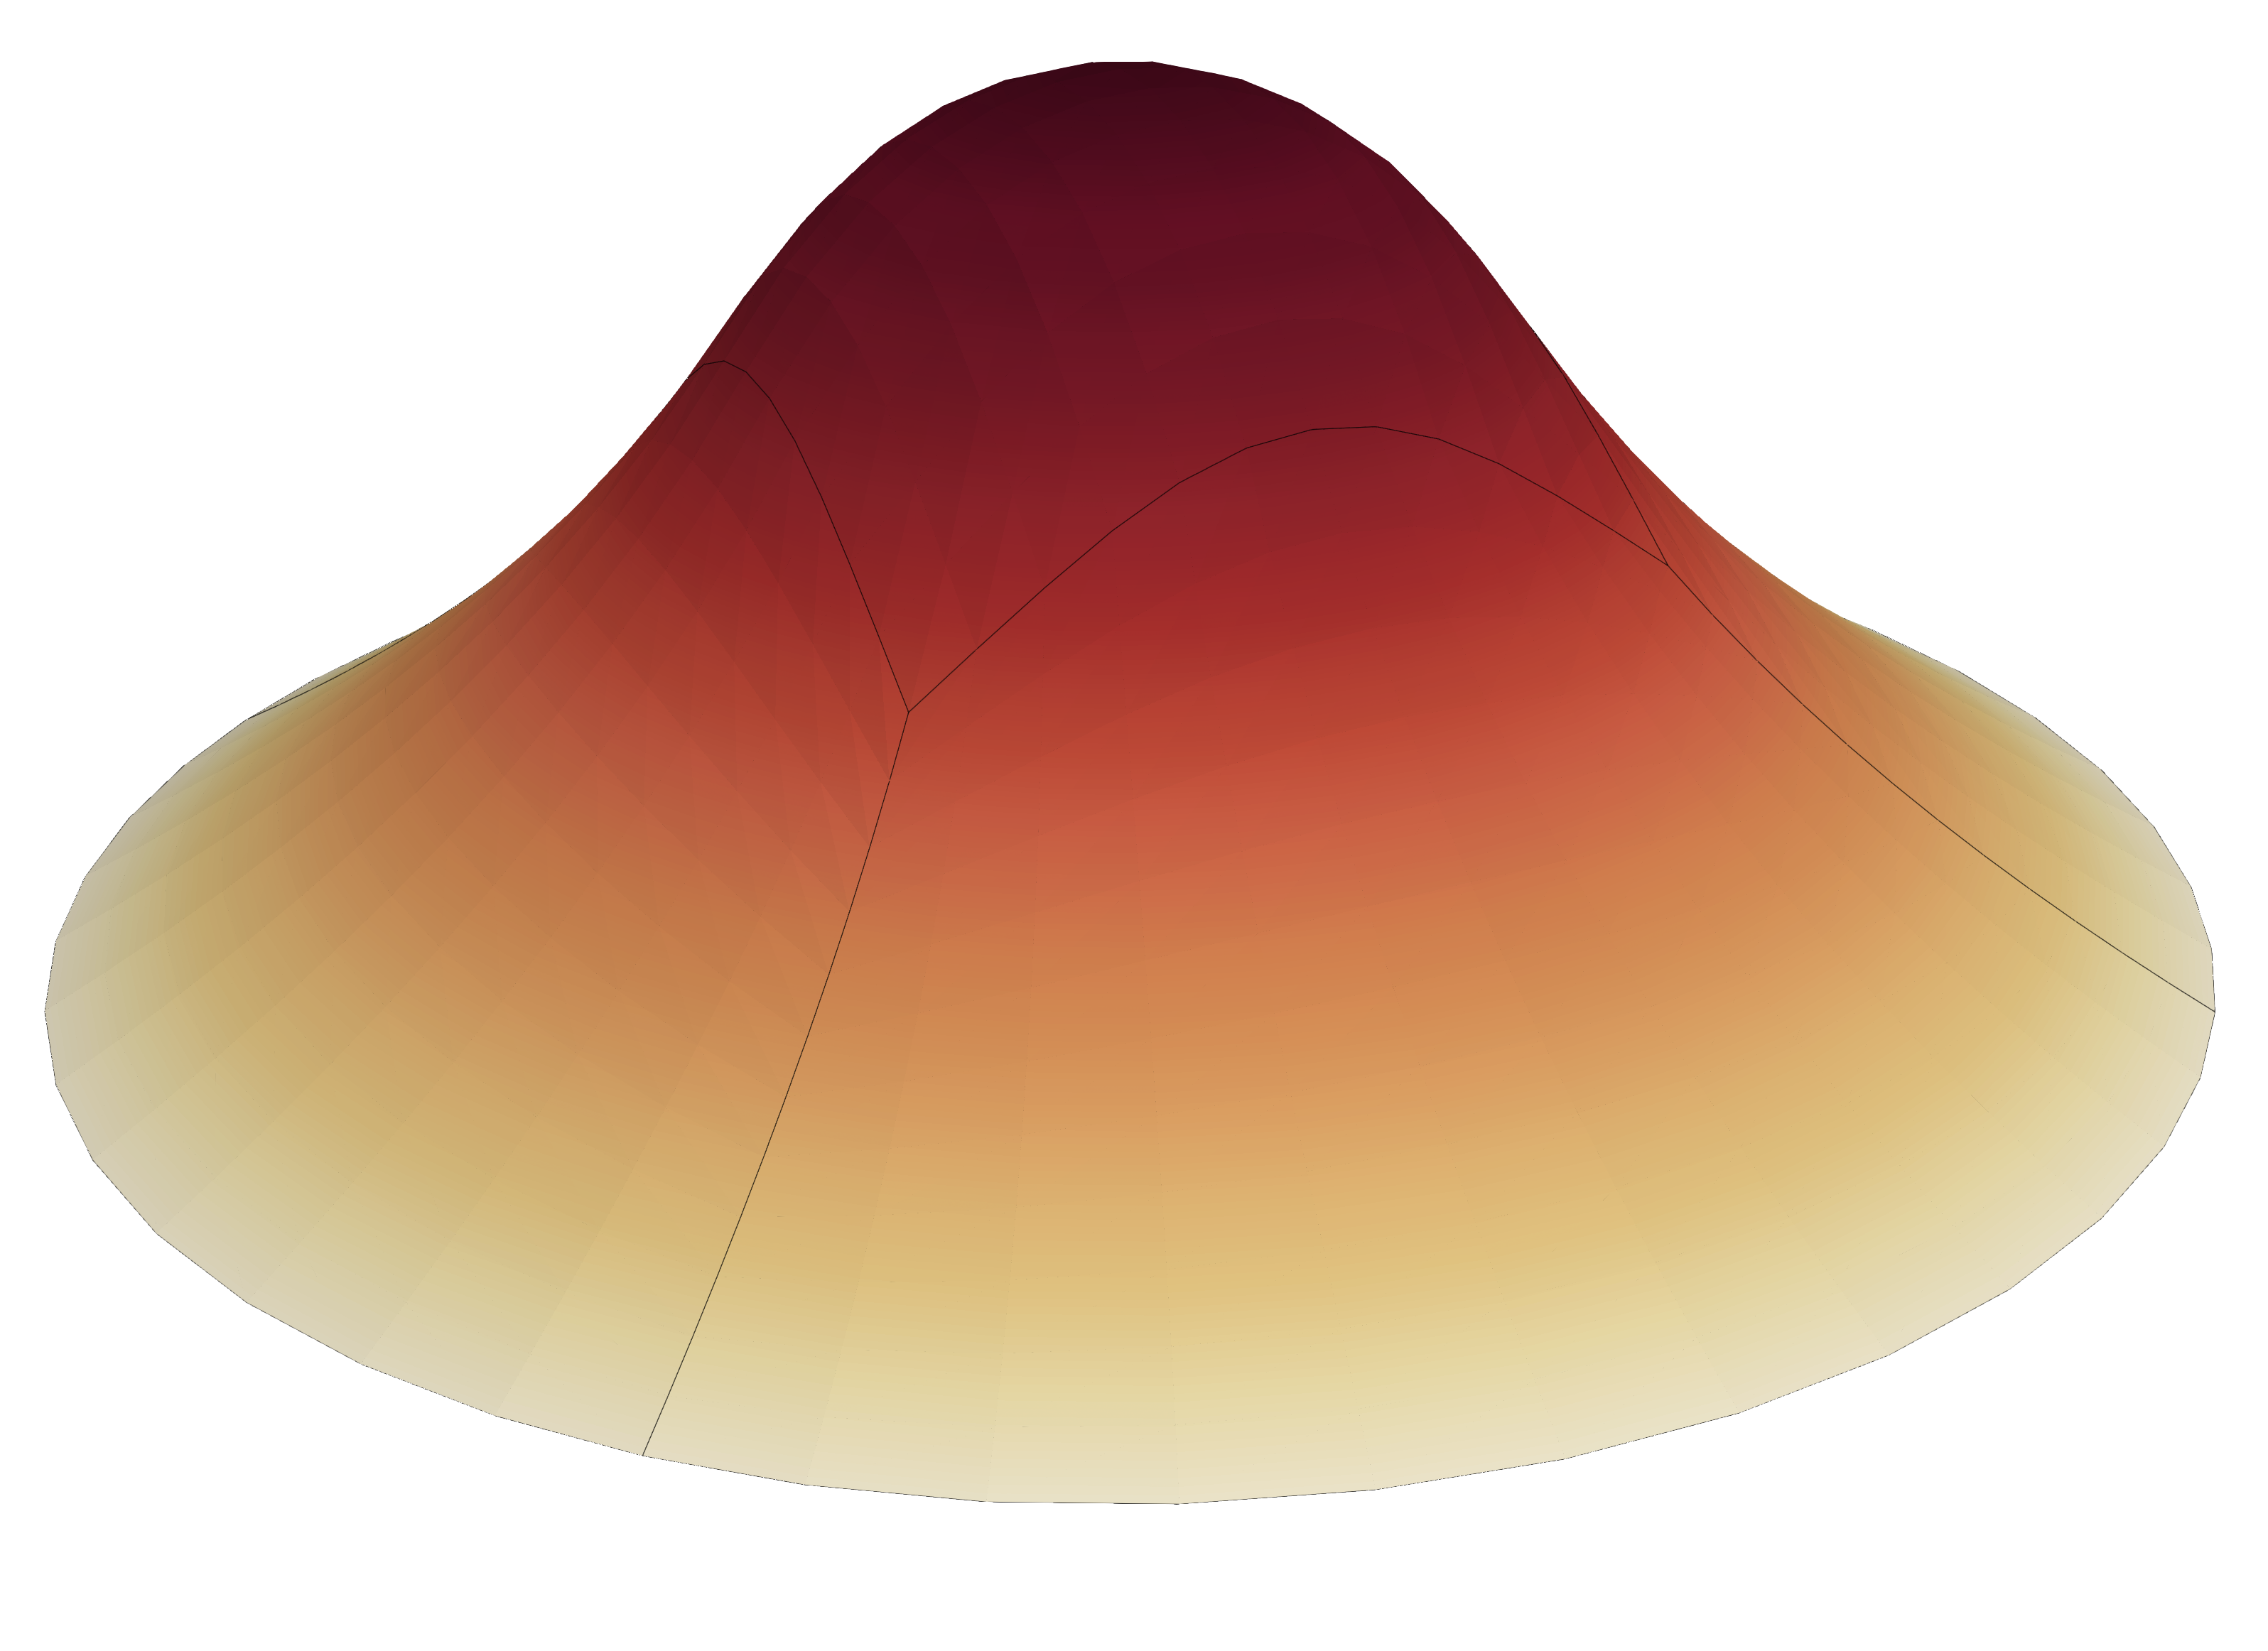
\includegraphics[clip=true, trim = 0cm 2cm 0cm 1cm, width=0.5\linewidth]{Figures/ObstacleExperiment4_uh_alt}
			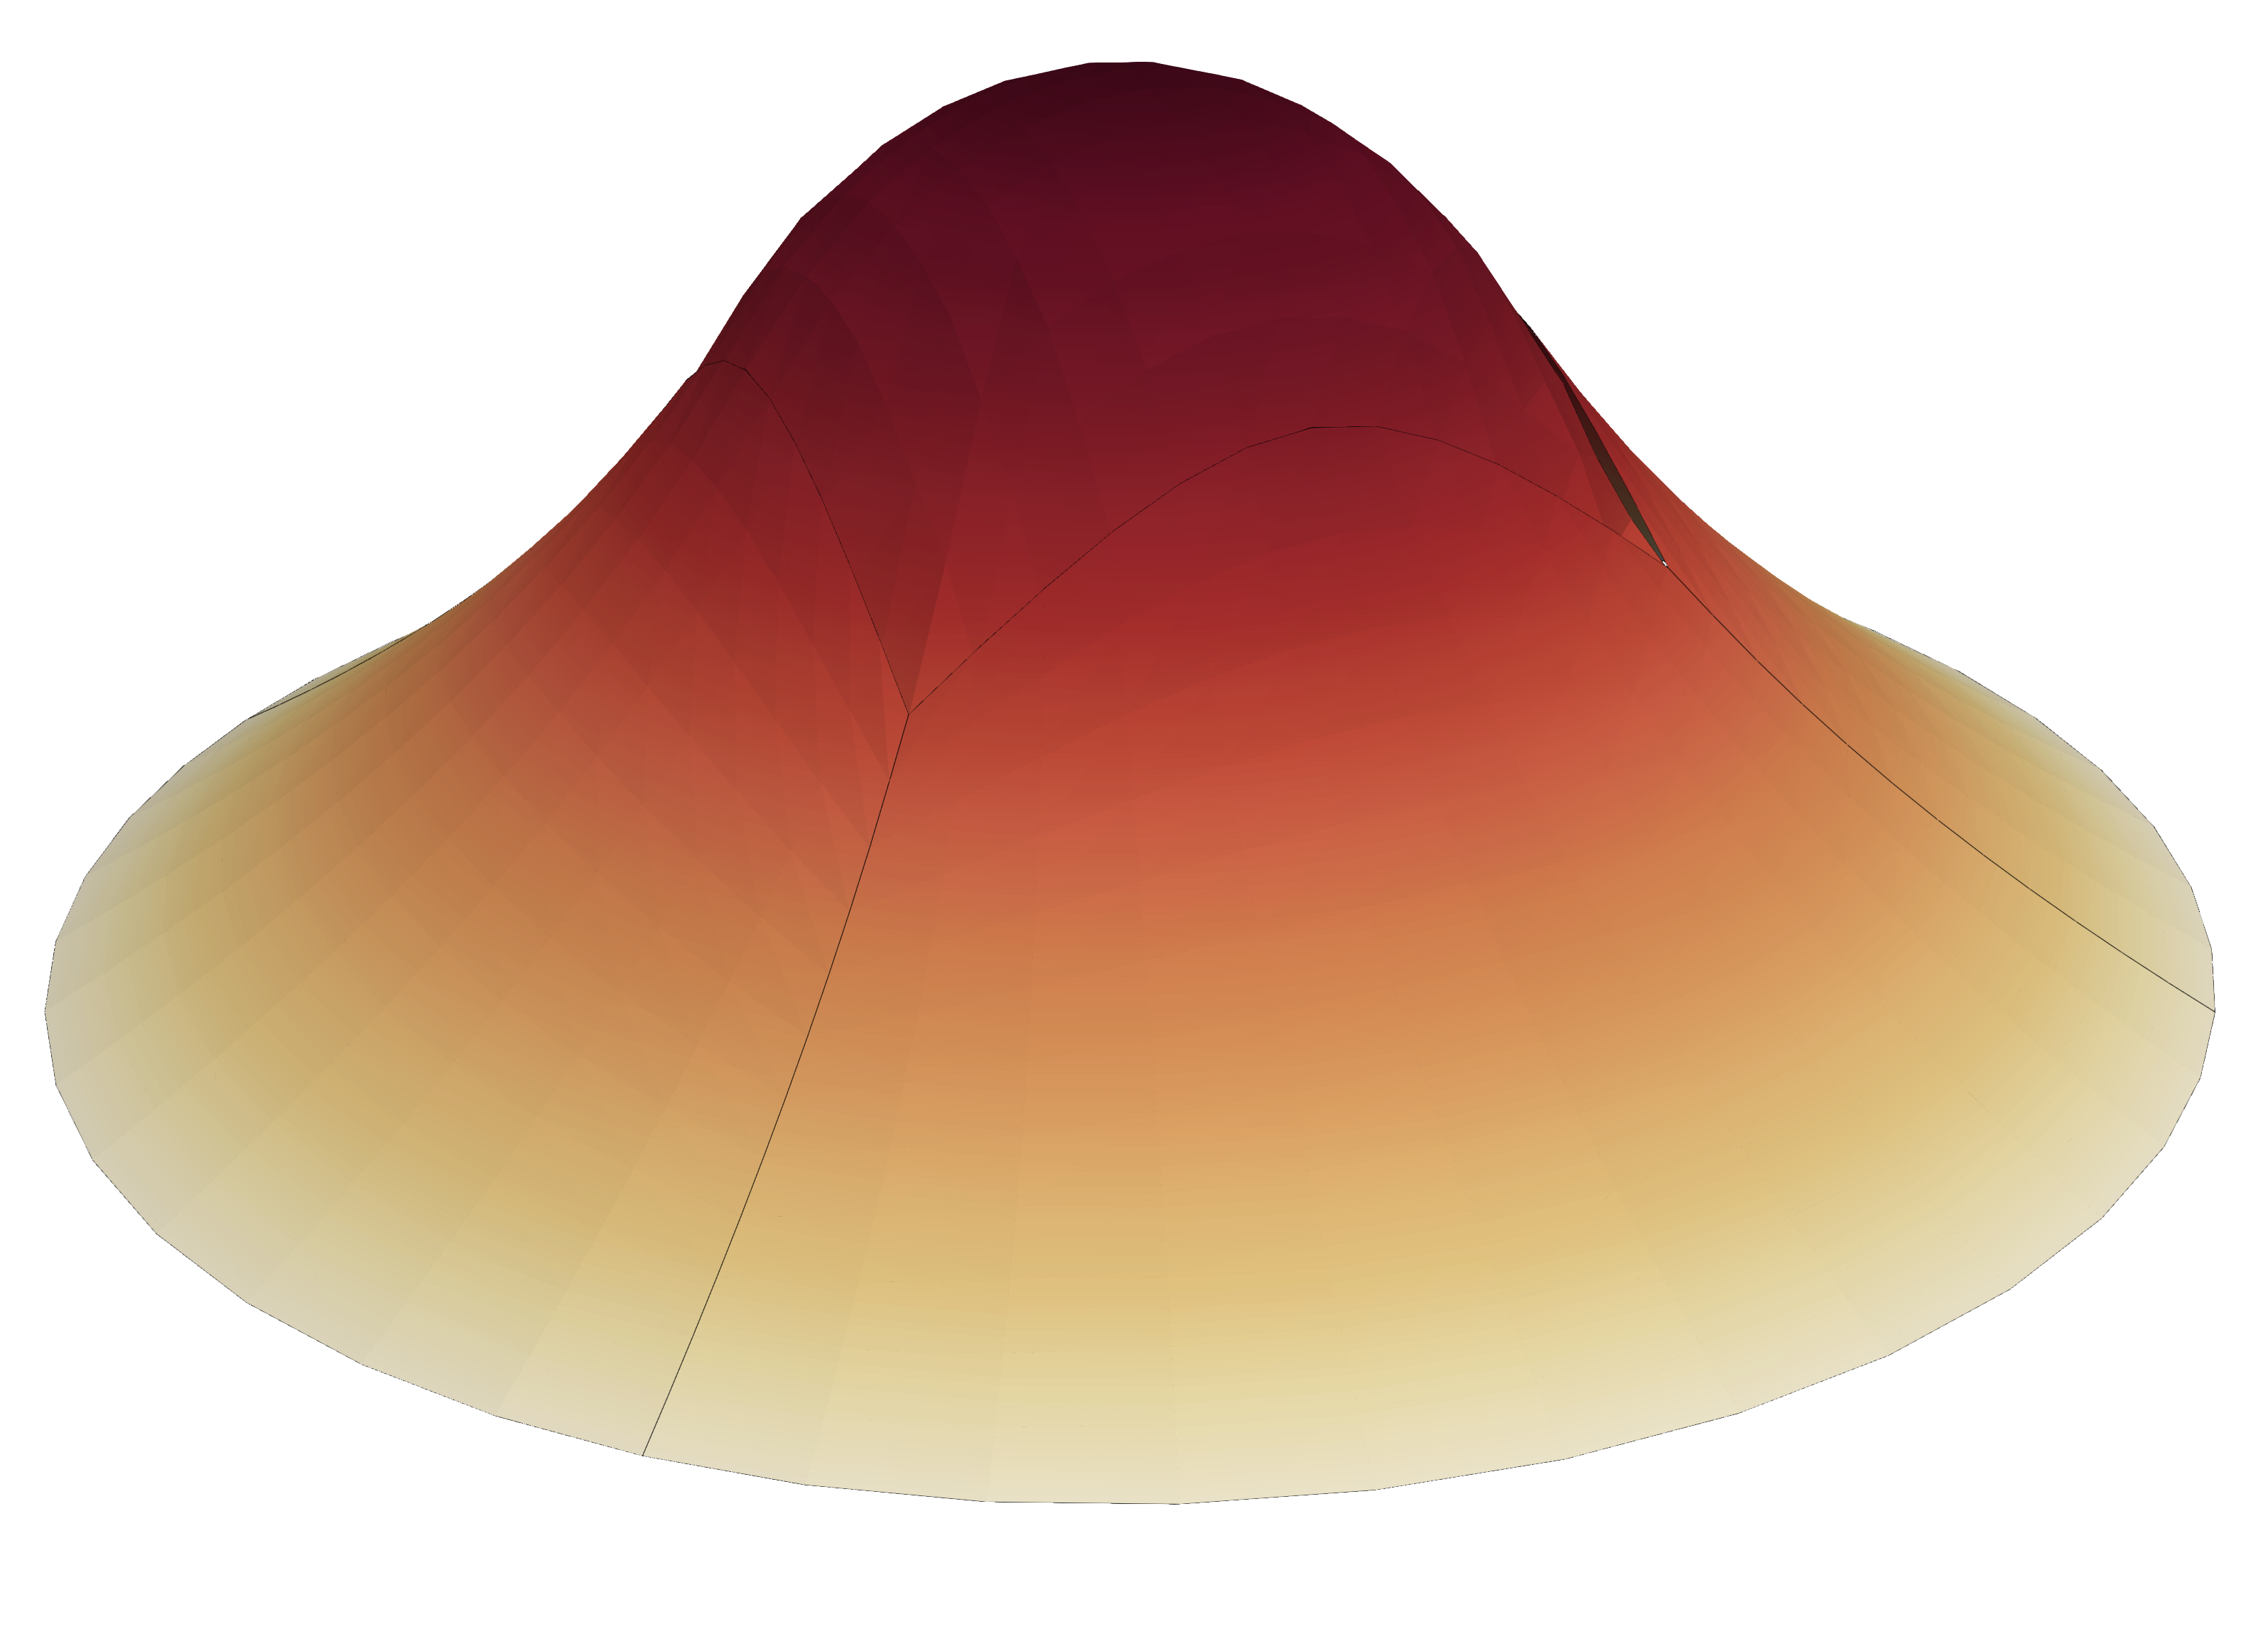
\includegraphics[clip=true, trim = 0cm 1cm 0cm 2cm, width=0.5\linewidth]{Figures/ObstacleExperiment4_uh_tilde_alt.png}
		\end{minipage}%
		\begin{minipage}[c]{0.075\textwidth}
			\centering
			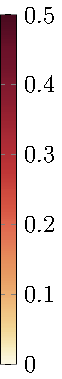
\includegraphics[width=\linewidth]{Figures/tikz/FEniCS_plots/example4/colorbar/colorbar5.pdf}
		\end{minipage}%
		\\
		Very high order ($p=12$) proximal Galerkin solutions $u_h$ (top) and $\tilde{u}_h$ (bottom)
	\end{minipage}
	\caption{
	Spherical obstacle.
	Benchmark obstacle problem.
	Left: Diagram of the problem set-up.
	% We solve $\min_{u\in H^1_0}~ \|\nabla u\|^2 \text{~subject to~} u \geq \phi \text{~a.e.}$, where $\phi(x)$ defines a sphere of radius $0.5$ centered at the origin.
	Right: Five-element proximal Galerkin solutions $u_h$ and $\tilde{u}_h$.
	% obtained with MFEM \cite{anderson2021mfem}.
	% To the best of our knowledge, this is the highest order that has been used in the literature to solve this problem.
	% The code to reproduce this result is available at \cite{Keith2023ObstacleCode}.
	\label{fig:ObstacleSphere}}
\end{figure}
\end{frame}

\begin{frame}\frametitle{Experiment 3: Results}
\begin{table}
\centering
\footnotesize
\renewcommand{\arraystretch}{1.3}
\begin{tabular}{ |c|c|c|c|c|c|c| }
 % \cline{3-8}
 \hhline{|>{\arrayrulecolor{white}}-->{\arrayrulecolor{black}}|-----|}
 \multicolumn{2}{c|}{} & \multicolumn{5}{c|}{\cellcolor{lightgray!15} \small\raisebox{5pt}{\phantom{f}} Primal errors $\|u - u_h^{k}\|_{H^1(\Omega_2)}$ for $p=1$ \raisebox{5pt}{\phantom{f}}}\\[3pt]
 \hline
 \rowcolor{lightgray!15}
 $k$ & Linear solves & $h_2/8$ & $h_2/16$ & $h_2/32$ & $h_2/64$ & $h_2/128$ \\
 \hline
 \cellcolor{lightgray!05} 1 & \cellcolor{lightgray!01} 3 & $2.72\cdot 10^{-1}$ & $2.70\cdot 10^{-1}$ & $2.70\cdot 10^{-1}$ & $2.70\cdot 10^{-1}$ & $2.70\cdot 10^{-1}$ \\
 \cellcolor{lightgray!05} 2 & \cellcolor{lightgray!01} 1 & $1.37\cdot 10^{-1}$ & $1.38\cdot 10^{-1}$ & $1.38\cdot 10^{-1}$ & $1.38\cdot 10^{-1}$ & $1.38\cdot 10^{-1}$ \\
 \cellcolor{lightgray!05} 3 & \cellcolor{lightgray!01} 1 & $3.62\cdot 10^{-2}$ & $3.33\cdot 10^{-2}$ & $3.31\cdot 10^{-2}$ & $3.31\cdot 10^{-2}$ & $3.31\cdot 10^{-2}$ \\
  \vdots & \vdots & \vdots & \vdots & \vdots & \vdots & \vdots \\[4pt]
 \hline
 \rowcolor{lightgray!05}
 \multicolumn{2}{|c|}{\cellcolor{lightgray!15} Total iterations} & $11$ & $11$ & $11$ & $11$ & $11$ \\
 \hline
 \rowcolor{lightgray!05}
 \multicolumn{2}{|c|}{\cellcolor{lightgray!15} Total linear solves} & $13$ & $13$ & $13$ & $13$ & $13$ \\
 \hline
 \rowcolor{lightgray!05}
 \multicolumn{2}{|c|}{\cellcolor{lightgray!15} Final error} & $1.98\cdot 10^{-2}$ & $8.73\cdot 10^{-3}$ & $3.49\cdot 10^{-3}$ & $1.18\cdot 10^{-3}$ & $3.85\cdot 10^{-4}$ \\
 \hline
\end{tabular}
\caption{\label{tab:ObstableErrorsp1}
	Subproblem error, $\|u-u^k_h\|_{H^1(\Omega_2)}$, for various mesh sizes using $(\mathbb{Q}_2,\mathbb{Q}_{0}\text{-broken})$ discretization.
	We used $\alpha_k = 1$ for all $k=1,\ldots$ and stopped the algorithm when $\|u_h^{k} - u_h^{k-1}\|_{L^2(\Omega_2)} < 10^{-6}$.
}
\end{table}
\end{frame}

\section{Extensions of Proximal Galerkin}
\begin{frame}\frametitle{Nonsymmetric VI}
{\Large
{\color{Maroon}
What about variational inequalities that do not arise as energy minimization principles?
}
}
\end{frame}

\begin{frame}\frametitle{Ext. 1: Discrete Maximum Principle}
\begin{itemize}
\item
Let $\epsilon > 0$, $\beta \in \mathbb{R}^d$ be fixed, $f \in L^\infty(\Omega)$, and $g \in H^1(\Omega) \cap C(\overline{\Omega})$. 
\item The solution $u$ to the advection diffusion equation should satisfy a maximum principle on the continuous and \textbf{discrete} level:
\begin{equation}
\label{eq:AdvectionDiffusionEquation}
	-\epsilon\Delta u + \beta\cdot\nabla u = f
	\quad \text{in~} \Omega,
	\qquad
	u = g \quad \text{on~} \partial\Omega
	\,,
\end{equation}
\item By rewriting \eqref{eq:AdvectionDiffusionEquation} as a variational inequality, we can develop a Proximal Galerkin scheme.
\item There are (many) details in the paper including a ``binary entropic Poisson equation'', an implementable algorithm, further pairs of tailored FE spaces for the new saddle point problems.
\end{itemize}
\end{frame}

\begin{frame}\frametitle{Ext. 1: Discrete Maximum Principle}
\begin{figure}
	\centering
	\begin{minipage}{0.3\textwidth}
	\small
		\centering
		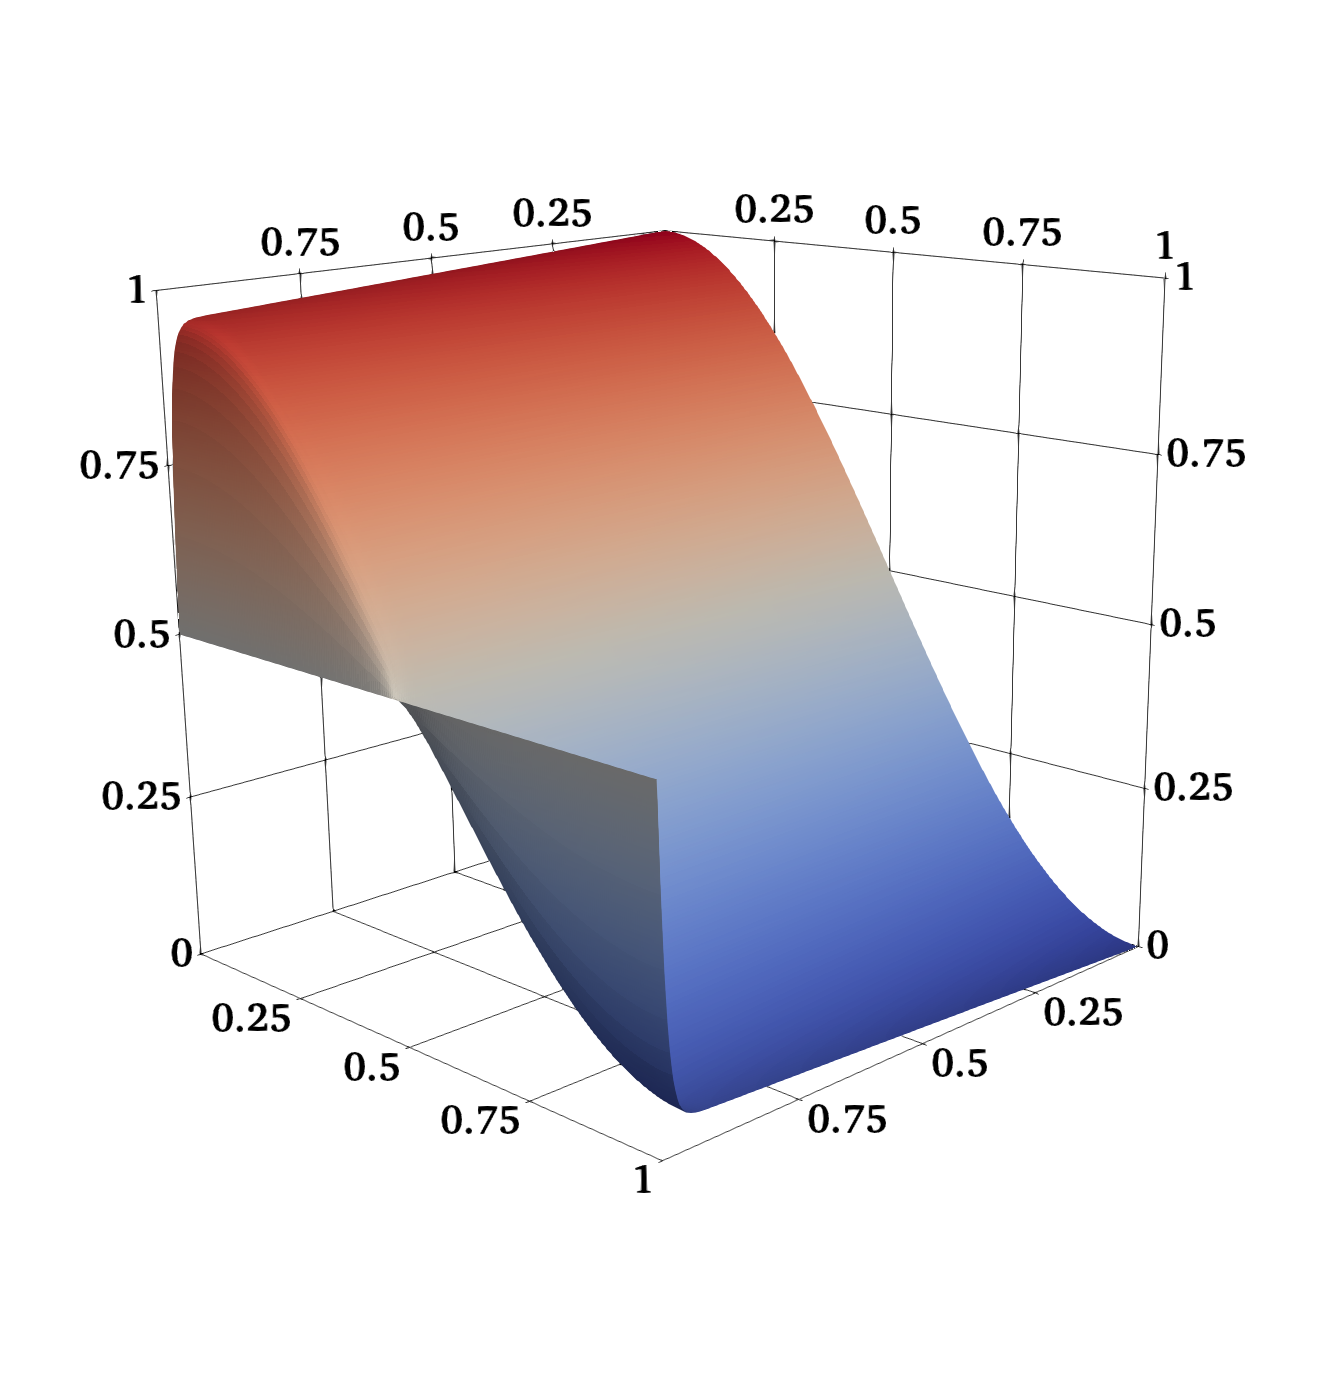
\includegraphics[width=\linewidth]{Figures/advection_diffusion_u_exact.png}
		\\
		Exact solution $u$
	\end{minipage}%,
	\
	\begin{minipage}{0.03\textwidth}
	\small
		\centering
		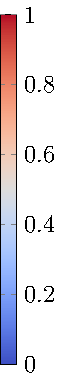
\includegraphics[width=\linewidth]{Figures/advection_diffusion_colorbar.pdf}
		\\[1.5em]
		~
	\end{minipage}%
	~~~
	\begin{minipage}{0.3\textwidth}
	\small
		\centering
		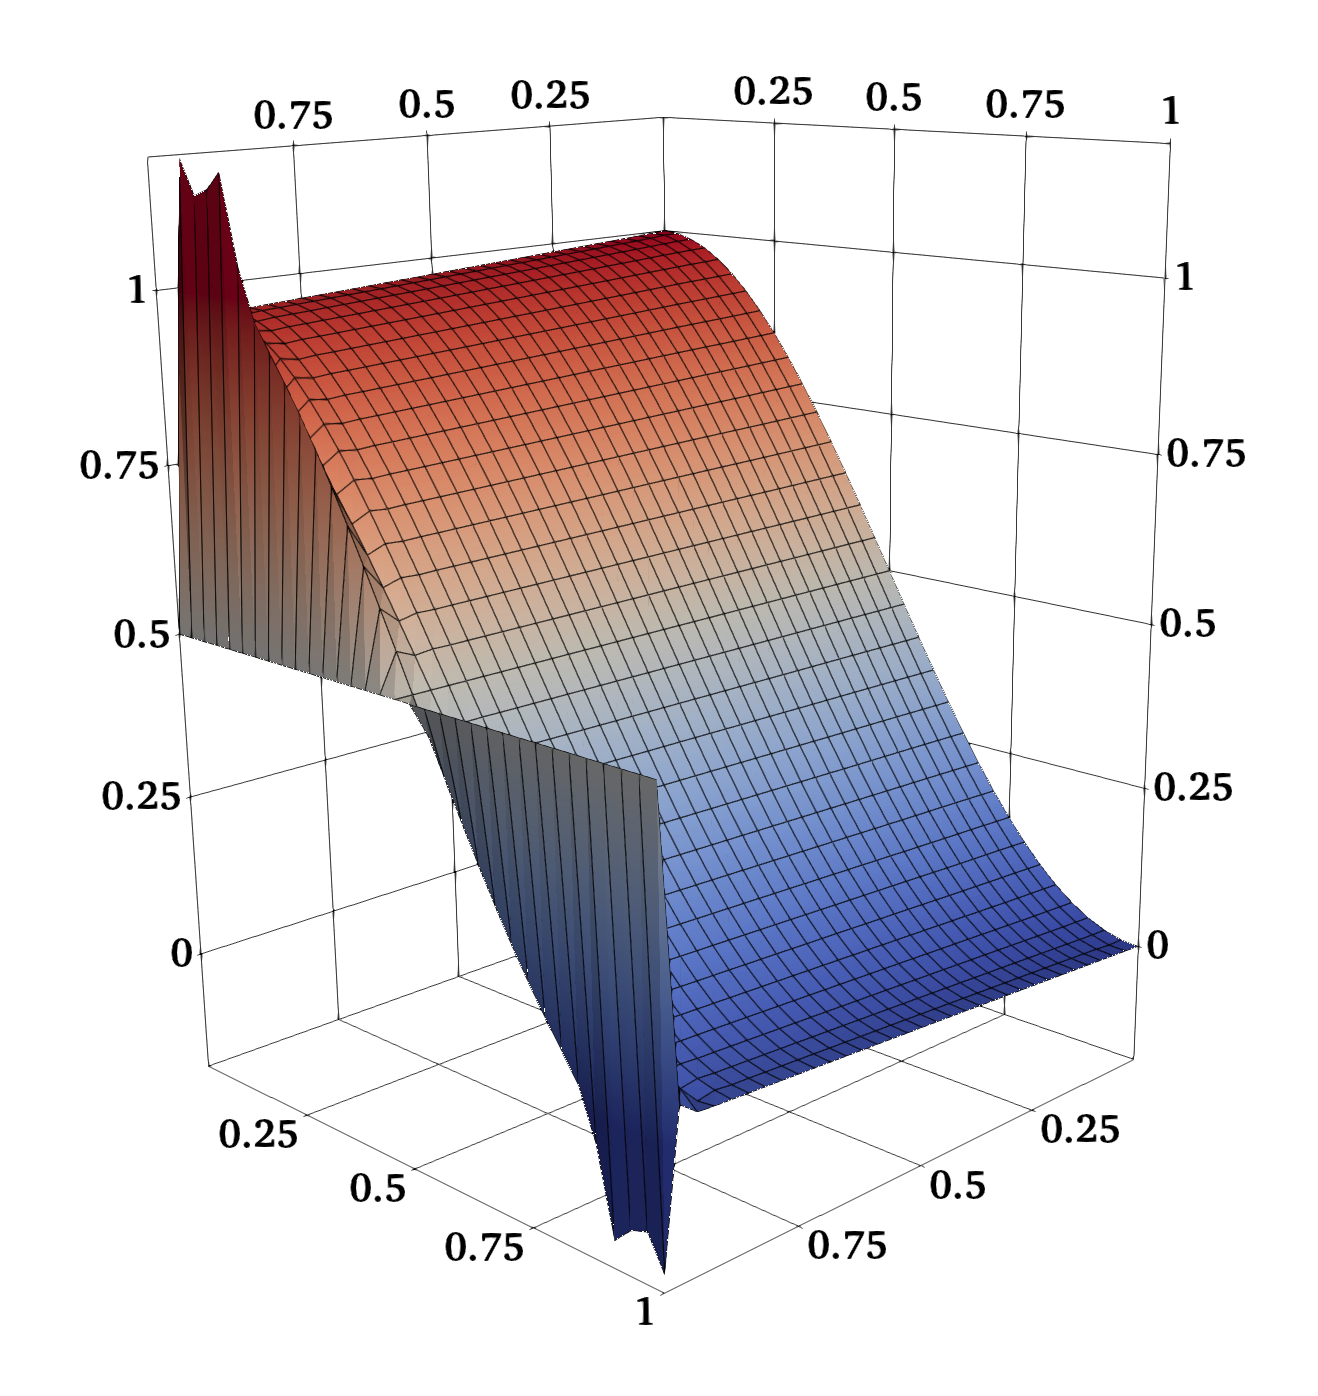
\includegraphics[width=\linewidth]{Figures/advection_diffusion_u_h.png}
		\\
		FEM solution
	\end{minipage}%,
	~
	\begin{minipage}{0.3\textwidth}
	\small
		\centering
		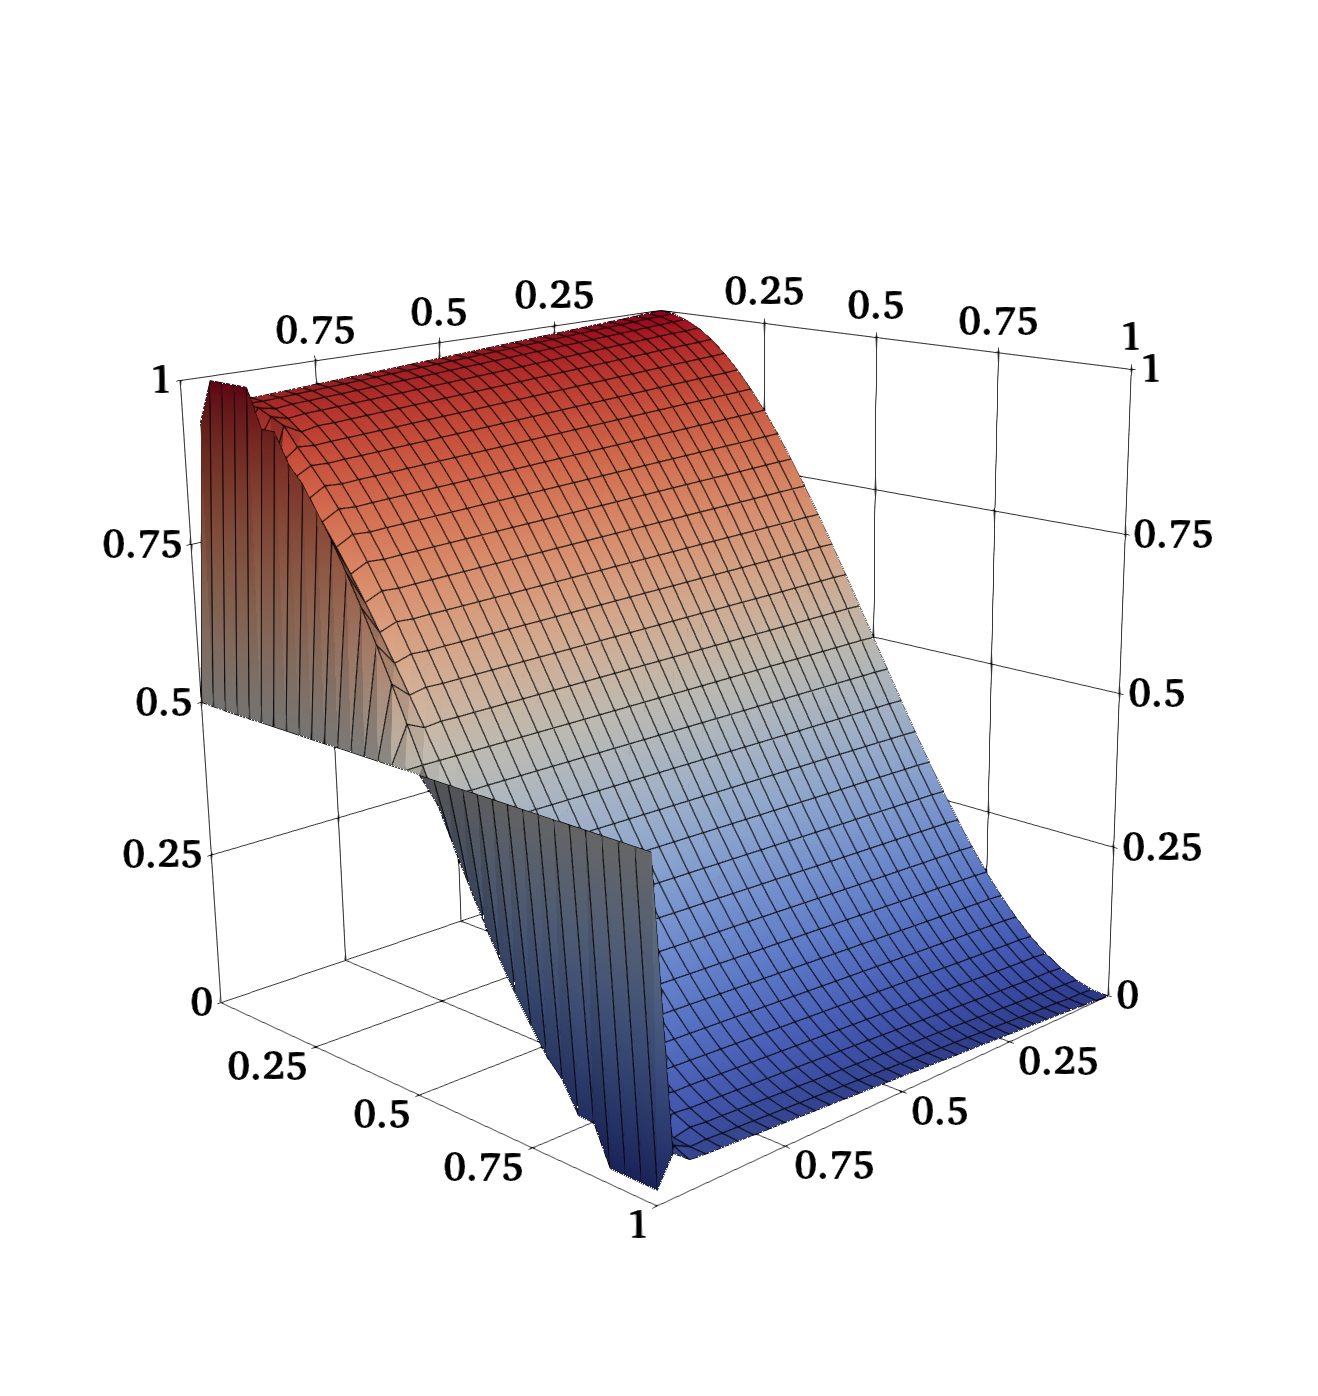
\includegraphics[width=\linewidth]{Figures/advection_diffusion_utilde.png}
		\\
		Proximal Galerkin solution $\tilde{u}_h$
	\end{minipage}%
	\caption{
	Erikkson--Johnson problem with $\epsilon = 10^{-2}$.
	(l):  Exact solution.
	(c): A first-order Bubnov--Galerkin numerical solution that clearly violates the strong maximum principle $0 \leq u(x) \leq 1$.
	(r): $(\mathbb{Q}_1,\mathbb{Q}_1)$-proximal Galerkin solution $\tilde{u}_h = \sigmoid(\psi_h)$ satisfies the strong maximum principle, by construction.
	% These results were obtained with our MFEM implementation \cite{ZenodoCode}.
%	These results can be reproduced by running the MFEM code \texttt{advection\_diffusion.cpp} available at \cite{ZenodoCode}.
	% using $\rho = 1.0$ and $\alpha_k = 0.01$, $k = 1,2,\ldots$
	\label{fig:EJProblem}}
\end{figure}
\end{frame}

\begin{frame}\frametitle{Nonconvex Problems}
{\Large
{\color{Maroon}
What about nonconvex variational problems?
}
}
\end{frame}

\begin{frame}\frametitle{Ext. 2.: Topology Optimization}
\textbf{Find a material distribution with maximum flexibility and a fixed volume}:
\begin{equation}
\label{eq:elastic_compliance_objective}
    \min_{\rho \in L^{\infty}(\Omega)} \ \
    \left\{
    \,
    \widehat{F}(\mathbf{u},\rho)
    =
    \int_{ \Omega} \mathbf{u}\cdot\mathbf{f} \dd \bm{x}
    \,
    \right\}
    \, ,
\end{equation}
subject to the constraints
\begin{equation}
\label{eq:elastic_compliance_constraints}
\left\{\,\,
\begin{gathered}
    -\mathrm{Div} \left( r(\tilde{\rho})\,\bm{\sigma} \right) = \mathbf{f}
    ~~ \text{in }\Omega
    \quad\text{with}\quad
    \mathbf{u} = 0
    ~~\text{on }\Gamma_0
    \,,
    \quad
    \bm{\sigma} \mathbf{n} = 0
    ~~ \text{on }\partial\Omega \setminus \Gamma_0
    \,,
    \\
    -\epsilon^2\Delta \tilde{\rho} + \tilde{\rho}
	= \rho
	~~ \text{in }\Omega
	\quad\text{with}\quad
	\nabla \tilde{\rho}\cdot \mathbf{n} = 0
	~~ \text{on }\partial\Omega
    \,,
    \\
    \int_\Omega \rho(\bm{x}) \dd\bm{x}
    = \theta |\Omega|
    \,,\quad
    0 \leq \rho
    \leq 1
    \,,\quad
    r(\tilde{\rho})
    = \underline{\rho}+ \tilde{\rho}^3 (1-\underline{\rho})
    \,,
\end{gathered}
\right.
\end{equation}
%\end{subequations}
where $\epsilon > 0$ is a \emph{length scale} and $0 < \theta < 1$ is the desired {volume fraction}, which constrains the amount of the domain $\Omega$ occupied by the design.
\end{frame}

\begin{frame}\frametitle{Ext. 2: Topology Optimization}
\begin{figure}
\centering
	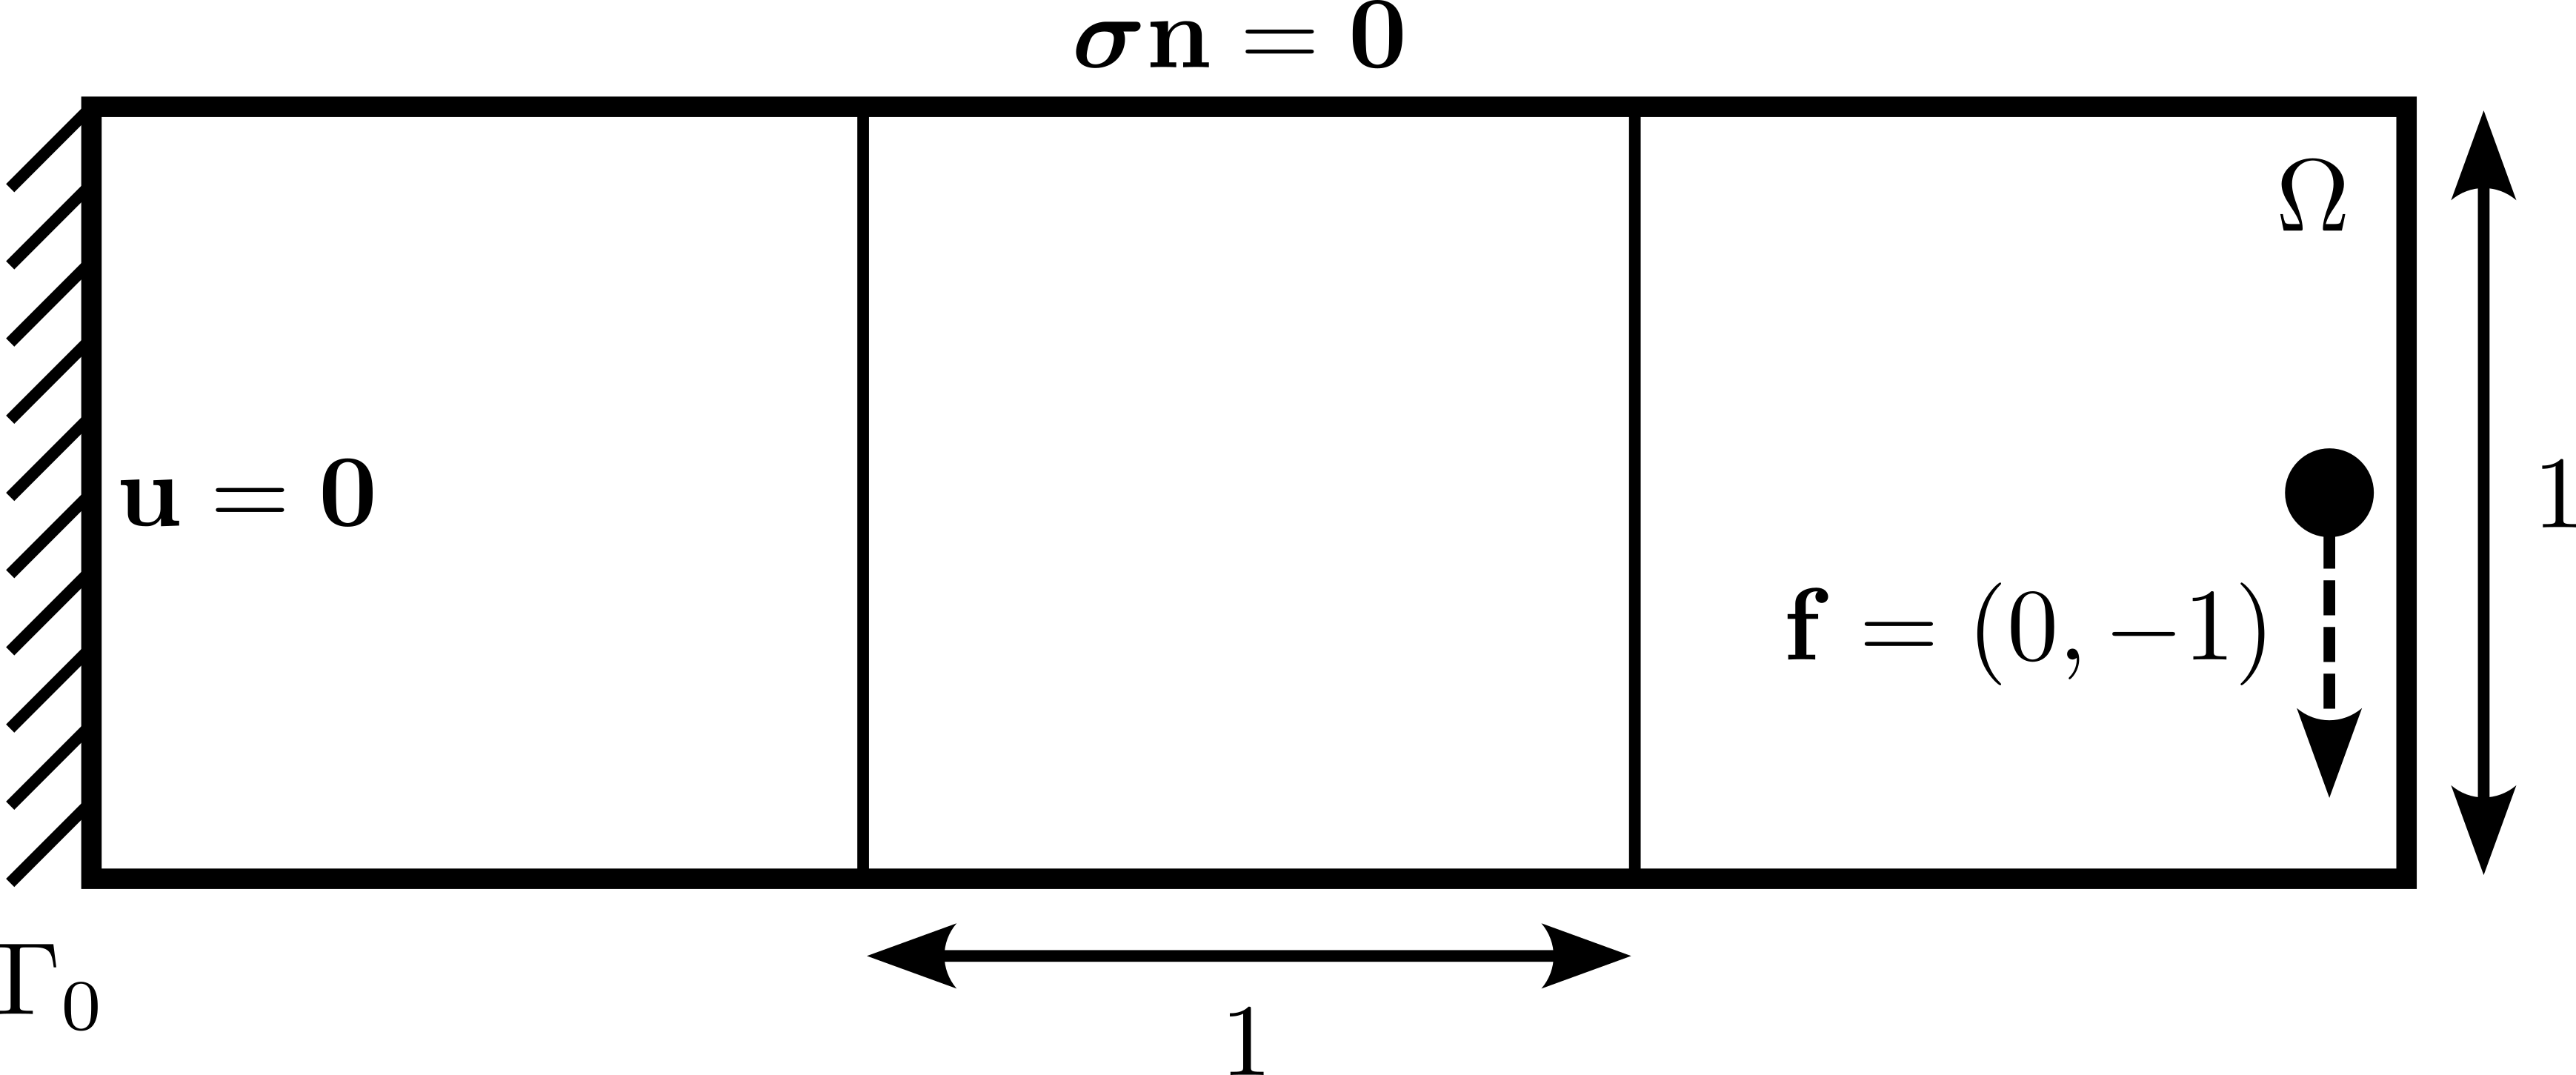
\includegraphics[width=7.5cm]{Figures/Cantilever_mesh.png}
	\caption{
	The design domain $\Omega$ for the cantilever beam problem with corresponding boundary conditions and three-element initial mesh with length $h_0 = 1$.
	\label{fig:ElasticCompliance_mesh}}
\end{figure}
\end{frame}

\begin{frame}\frametitle{Mirror Descent}
\begin{itemize}
\item Like proximal point, but replace the objective with its linearization.
\end{itemize}
{\tiny
\begin{algorithm2e}[H]
\DontPrintSemicolon
	\caption{\label{alg:TopologyOptimization}
	Entropic mirror descent for topology optimization.
	}
	\SetKwInOut{Input}{Input}
	\SetKwInOut{Output}{Output}
	\BlankLine
	\Input{
	Initial latent variable $\rho^0 \in L^\infty(\Omega)$, sequence of step sizes $\alpha_k>0$, increment tolerance $\mathtt{itol.} > 0$, and normalized tolerance $\mathtt{ntol.} > 0$.}
	\Output{Optimized material density $\overline{\rho} = \sigmoid(\psi^k)$.}
	\BlankLine
	Initialize $k = 0$.\;
	\While{$\|\sigmoid(\psi^k) - \sigmoid(\psi^{k-1})\|_{L^1(\Omega)} > \min\{\alpha_k\, \mathtt{ntol.},\mathtt{itol.}\}$}
	% \For{$k = 0,1,2,\ldots$}
	{
		\tcp*[l]{Latent space gradient descent}
		Assign $\psi^{k+1/2} \leftarrow  \psi^{k} - \alpha_{k+1} \nabla F(\sigmoid(\psi^k))$.\;
		\tcp*[l]{Compute Lagrange multiplier}
		Solve for $c \in \mathbb R$ such that $\int_\Omega \sigmoid(\psi^{k+1/2} + c) \dd x = \theta |\Omega|$.\;
		\tcp*[l]{Latent space feasibility correction}
		Assign $\psi^{k+1} \leftarrow  \psi^{k+1/2} + c$.\;
		Assign $k \leftarrow k+1$.\;
	}
\end{algorithm2e}
}
\end{frame}

\begin{frame}\frametitle{Ext. 2: Results}
\begin{figure}
\centering
	\centering
	\begin{minipage}[c]{0.96\textwidth}
		\begin{minipage}[c]{0.32\textwidth}
		\small
			\centering
			
\includegraphics[width=\textwidth]{Figures/TopOpt/alpha25/Cantilever0.png}
			\\[3pt]
			$k = 0$
		\end{minipage}
		\begin{minipage}[c]{0.32\textwidth}
		\small
			\centering
			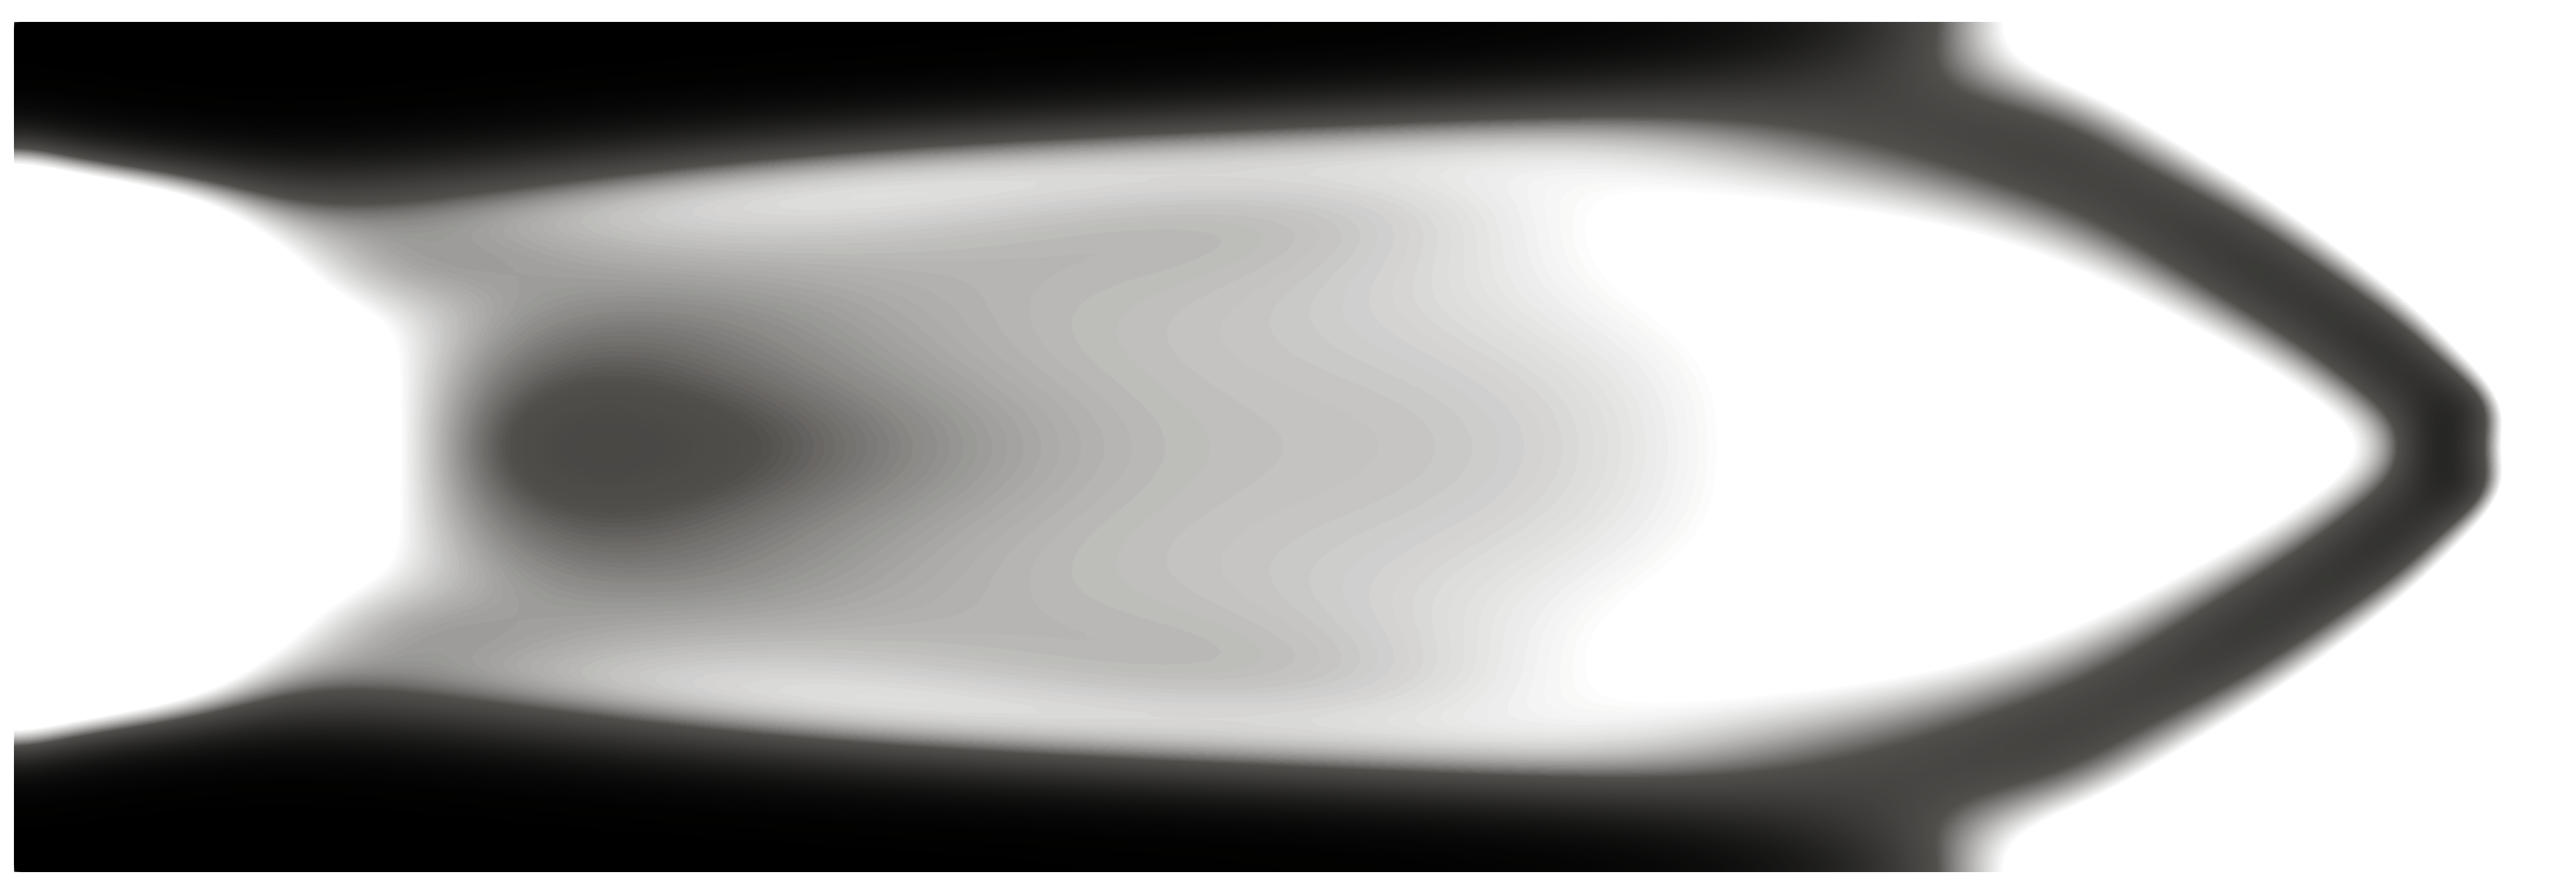
\includegraphics[width=\textwidth]{Figures/TopOpt/alpha25/Cantilever6.png}
			\\[3pt]
			$k = 6$
		\end{minipage}
		\begin{minipage}[c]{0.32\textwidth}
		\small
			\centering
			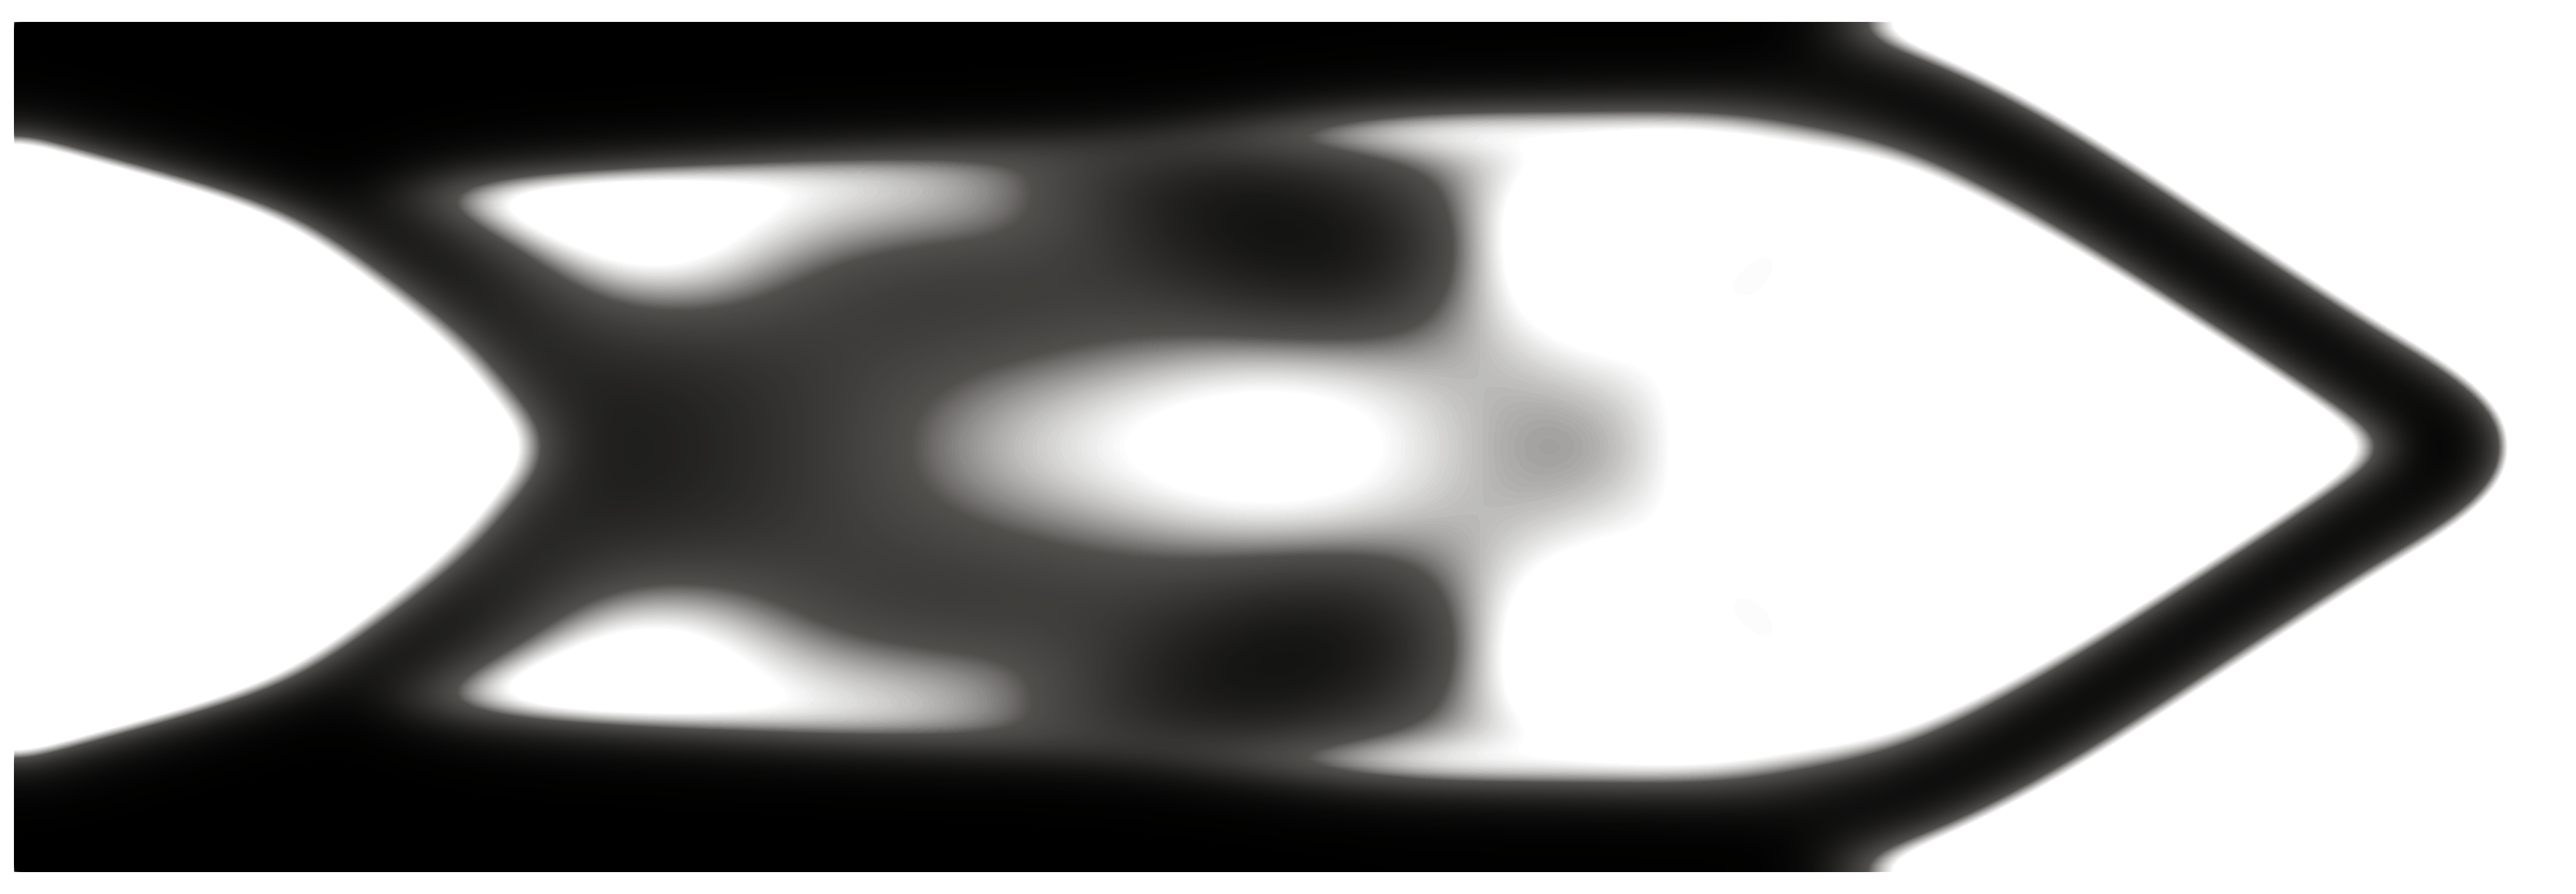
\includegraphics[width=\textwidth]{Figures/TopOpt/alpha25/Cantilever12.png}
			\\[3pt]
			$k = 12$
		\end{minipage}
		\\[7pt]
		\begin{minipage}[c]{0.32\textwidth}
		\small
			\centering
			
\includegraphics[width=\textwidth]{Figures/TopOpt/alpha25/Cantilever18.png}
			\\[3pt]
			$k = 18$
		\end{minipage}
		\begin{minipage}[c]{0.32\textwidth}
		\small
			\centering
			
\includegraphics[width=\textwidth]{Figures/TopOpt/alpha25/Cantilever24.png}
			\\[3pt]
			$k = 24$
		\end{minipage}
		\begin{minipage}[c]{0.32\textwidth}
		\small
			\centering
			
\includegraphics[width=\textwidth]{Figures/TopOpt/alpha25/Cantilever29.png}
			\\[3pt]
			$k = 29$ (final)
		\end{minipage}
	\end{minipage}
	\begin{minipage}[c]{0.032\textwidth}
		\centering
		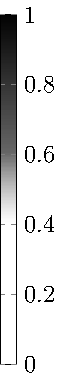
\includegraphics[width=\textwidth]{Figures/TopOpt/colorbar/colorbar_bw.pdf}
		\\[4pt]~
	\end{minipage}
	% \begin{minipage}[c]{0.96\textwidth}
	% 	\begin{minipage}[c]{0.32\textwidth}
	% 	\small
	% 		\centering
	% 		
\includegraphics[width=\textwidth]{Figures/TopOpt/alpha25/Cantilever0.png}
	% 		\\[3pt]
	% 		$k = 0$
	% 	\end{minipage}
	% 	\begin{minipage}[c]{0.32\textwidth}
	% 	\small
	% 		\centering
	% 		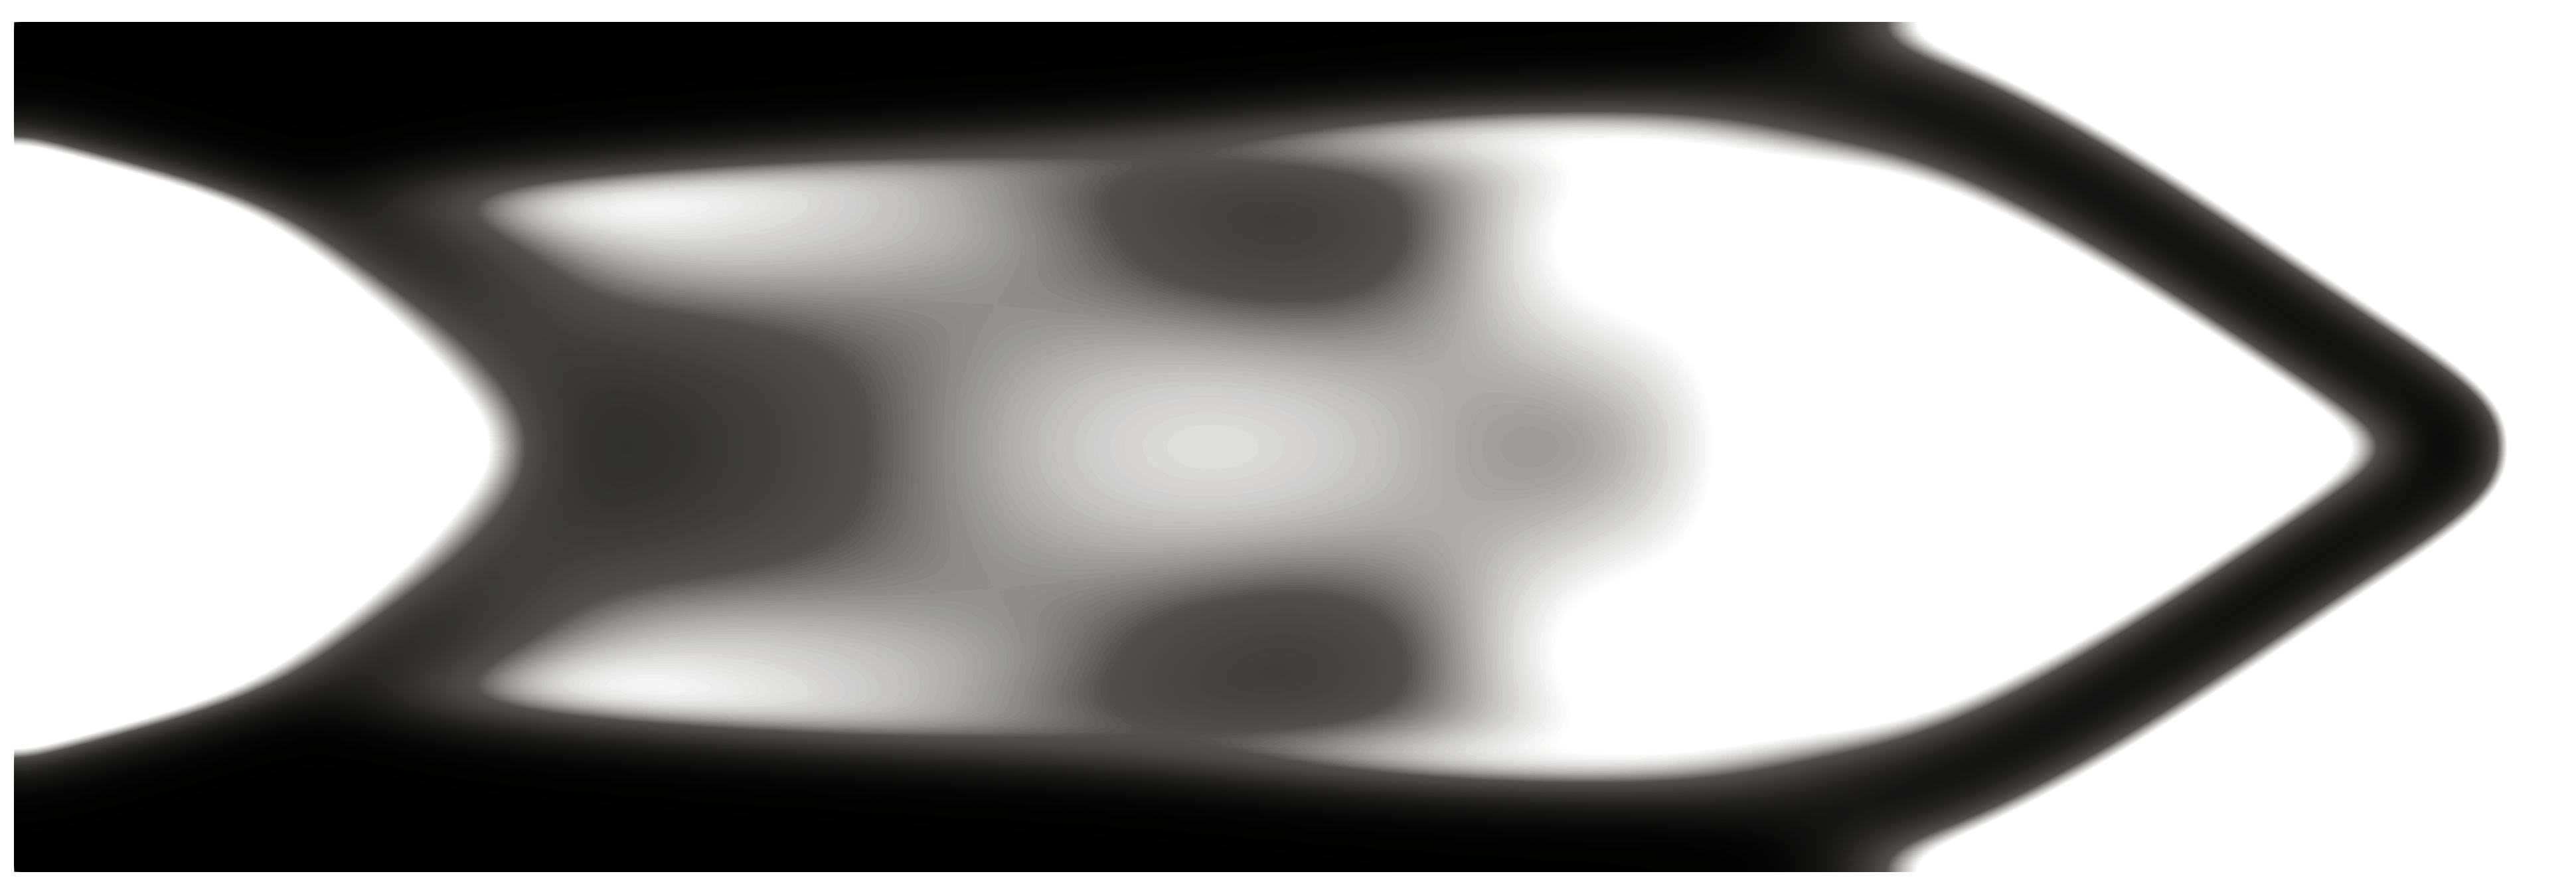
\includegraphics[width=\textwidth]{Figures/TopOpt/alpha25/Cantilever10.png}
	% 		\\[3pt]
	% 		$k = 10$
	% 	\end{minipage}
	% 	\begin{minipage}[c]{0.32\textwidth}
	% 	\small
	% 		\centering
	% 		
\includegraphics[width=\textwidth]{Figures/TopOpt/alpha25/Cantilever20.png}
	% 		\\[3pt]
	% 		$k = 20$
	% 	\end{minipage}
	% 	\\[7pt]
	% 	\begin{minipage}[c]{0.32\textwidth}
	% 	\small
	% 		\centering
	% 		
\includegraphics[width=\textwidth]{Figures/TopOpt/alpha25/Cantilever30.png}
	% 		\\[3pt]
	% 		$k = 30$
	% 	\end{minipage}
	% 	\begin{minipage}[c]{0.32\textwidth}
	% 	\small
	% 		\centering
	% 		
\includegraphics[width=\textwidth]{Figures/TopOpt/alpha25/Cantilever40.png}
	% 		\\[3pt]
	% 		$k = 40$
	% 	\end{minipage}
	% 	\begin{minipage}[c]{0.32\textwidth}
	% 	\small
	% 		\centering
	% 		
\includegraphics[width=\textwidth]{Figures/TopOpt/alpha25/Cantilever53.png}
	% 		\\[3pt]
	% 		$k = 53$ (final)
	% 	\end{minipage}
	% \end{minipage}
	% \begin{minipage}[c]{0.032\textwidth}
	% 	\centering
	% 	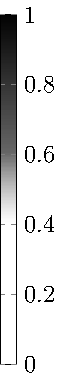
\includegraphics[width=\textwidth]{Figures/TopOpt/colorbar/colorbar_bw.pdf}
	% 	\\[4pt]~
	% \end{minipage}
	\caption{
	% Cantilever beam.
	Subsequence of material densities $\tilde{\rho}_h^k$ from~\Cref{alg:TopologyOptimization} for selected iterations $k$.
	Results obtained with problem parameters $\epsilon = 2\cdot 10^{-2}$ and $\theta = 0.5$; algorithm parameters $\mathtt{itol.} = 10^{-2}$, $\mathtt{ntol.} = 10^{-5}$, and $\alpha_k = 25k$; and discretization parameters $h = h_0/128$ and $p = 1$.
	\label{fig:ElasticCompliance_sequence}}
\end{figure}
\end{frame}

\section{The Latent Variable Proximal Point Method}
\begin{frame}\frametitle{Latent Variable Proximal Point}
{\Large
{\color{Maroon}
What is really going on here?
}
}
\end{frame}

\begin{frame}\frametitle{A}

{\color{BlueViolet}\textbf{The LVPP Method:}} We seek a minimizer $\overline{u}$ of a smooth coercive functional $J$ over a closed convex subset $K$ of a Sobolev space $V$. We assume $K = \left\{v \in V \left| \Lambda v \in C \text{ a.e. } \Omega \right.\right\}$, $\Omega$ is an open bounded set, $\Lambda$ is a bounded linear operator into $L^2(\Omega)^n$ or $L^2(\Omega)^{n\times n}$, and $C$ is a nonempty closed convex subset of $\mathbb R^n$ or $\mathbb R^{n \times n}$. This enforces properties like non-negativity or boundedness of $\Lambda v$ almost everywhere on $\Omega$. 

Just as most PDEs do not admit analytical solutions in general, we require a numerical algorithm to approximate $\overline{u}$. The ideal method would be provably convergent, accurate, and exhibit low iteration complexity. Here, \textit{accuracy} refers to an achievable tolerance and \textit{complexity} to the number of steps required until a stopping criterion is fulfilled at that tolerance.  These infinite-dimensional problems have the added challenge that $V$ must be replaced by a finite-dimensional space $V_h$ in practice. This adds another desirable property: \textit{mesh-independence}, i.e. the iteration complexity for a fixed accuracy is independent of the discretization parameter $h$. Mesh-independence is deeply linked to the properties of $V,J,K$, and $\overline{u}$ itself at the \emph{continuous level} \cite{MWeiser_etal_2005} and entails an intricate analysis for constrained problems \cite{Hintermller2004}. For this reason, many researchers design and analyze algorithms for the infinite-dimensional problem. This is our perspective, as well.

As its name suggests, LVPP contains two essential components: The application of the classical \textbf{P}roximal \textbf{P}oint method introduced by Martinet \cite{BMartinet_1970}, though we follow the modern view from Teboulle et al., cf. \cite{MTeboulle_2018}, and the introduction of a \textbf{L}atent \textbf{V}ariable $\psi$. The latent variable is \textit{not} an approximation of a Lagrange multiplier. The generalized proximal point method for computing $\overline{u}$ is an iterative procedure that takes a penalty parameter $\alpha > 0$ and a previous iterate $v$ and returns a new approximation $u$ of $\overline{u}$  as the solution of the optimization problem: 
$
\min\{ J(u) + \alpha^{-1} D(\Lambda u,\Lambda v) : u \in K\}.
$ 
Here, $D$ is a Bregman distance, \cite{BREGMAN1967200},  which should capture the geometry of $C$ in a way that such subproblems can be considered \textit{unconstrained}. Bregman used a \textit{distance generating functional} $B$  to define $D$ as the local linearization error of $B$. Consequently, $u$ should solve the optimality system:
$
\alpha J'(u) + \Lambda^* B'(\Lambda u) = \Lambda^* B'(\Lambda v).
$
This still contains a potential difficulty in the term $B'(\Lambda u)$ and it is here that we first introduce the \textit{latent variable} $\psi$, which we set to be $\psi := B'(\Lambda u)$.  

\begin{wrapfigure}{R}{0.4\textwidth}
\vspace{-3ex}
%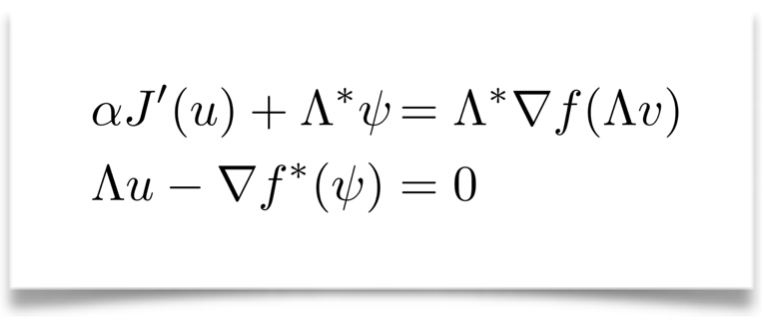
\includegraphics[width=\linewidth]{figures/lvpp-spp.png} 
\caption{The LVPP nonlinear saddle point subproblem. Similar saddle point formulations are \textbf{not} available in interior point, quadratic penalty, or augmented Lagrangian approaches.}
\label{fig:lvpp-spp}
\end{wrapfigure}

Similar to other algorithms that use a quadratic penalty term to relax $\Lambda u \in C$, $B$ should also be an integral functional so that $B'$ is a structured superposition (Nemitskii) operator, i.e. $[B'(y)](x) = \nabla f(y(x))$ for some real-valued mapping $f$.  The key here is to let $f$ be a \textit{Legendre} function whose domain \textit{coincides} with $C$. This unique property is not present in interior point, quadratic penalty, or augmented Lagrangian approaches. Introduced by Rockafellar in \cite{RTRockafellar_1970}, Legendre functions constitute a special class of convex functions that have the decisive property of $\nabla f$ forming a bijection from $\mathrm{int\, dom\,} f$ to $\mathrm{int\, dom\,} f^*$, where $f^*$ is the Fenchel conjugate of $f$, i.e. $(\nabla f)^{-1} = \nabla f^*$, where it is defined. This leads to the special nonlinear saddle point formulation in \Cref{fig:lvpp-spp}. I propose to call the unique superposition operators generated in this way \textit{Legendre-Nemitskii} operators. In \Cref{fig:lvpp-transform-table}, I formally compute the components that would arise for various sets $K$ and Legendre-Nemitskii operators.  After discretization, the solution $(\overline{u}_h,\overline{\psi}_{h})$ actually provides an additional (latent) solution: $\nabla f^*(\overline{\psi}_h)$, which by nature is always contained in $C$. This \textit{guarantees} a \textit{globally feasible discrete} approximation of $\Lambda \overline{u}$.

\begin{figure}[h]
%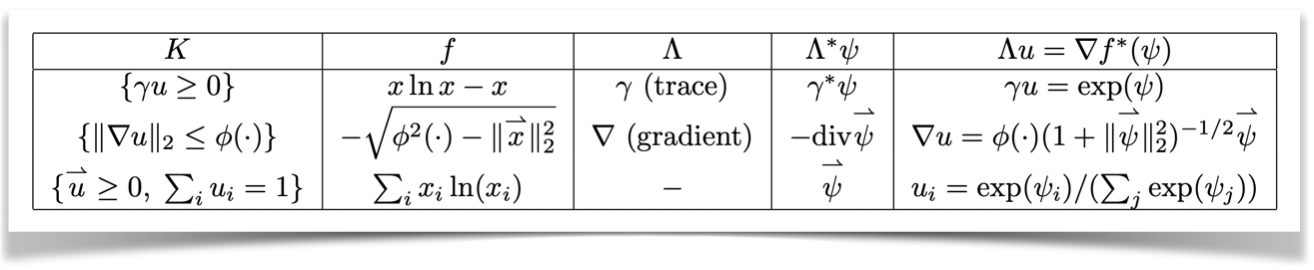
\includegraphics[width=\linewidth]{figures/lvpp-transform-table.png} 
\caption{Three examples of the versatility of Legendre-Nemitskii operators. $K$ is the original feasible set. $f$ is the finite-dimensional Legendre function. $\Lambda$ is the bounded linear operator in the composition. $\Lambda^* \psi$ is the derivative term after introducing the latent variable $\psi$ and $\Lambda u = \nabla f^*(\psi)$ is the nonlinear equation in the mixed formulation.}
\label{fig:lvpp-transform-table}
\end{figure}
By developing a specially tailored mixed finite element method to solve the LVPP saddle point subproblems, Brendan Keith and I introduced the Proximal Galerkin method mentioned earlier. Given the versatility of examples in \Cref{fig:lvpp-transform-table}, I strongly believe that the approach of combining LVPP with mixed finite element methods should be considered the canonical method for solving constrained variational problems with these and related structures.\medskip

\end{frame}
\end{document}



